%% ============================================================
%%  IEEE Transactions on Geoscience and Remote Sensing
%%
%%  Formatted using IEEEtran document class.
%%  Upload all .png/.jpg figures alongside this file.
%%  PRE-SUBMISSION CHECKLIST:
%%  - Verify all figures are >= 300 dpi (IEEE print requirement)
%%  - Convert line plots to PDF/EPS vector format where possible
%%  - DualTCN_Arch2.png should be vector (PDF) for best quality
%% ============================================================

\documentclass[journal]{IEEEtran}

%% ---- Packages ----------------------------------------------
\usepackage[utf8]{inputenc}
\usepackage[T1]{fontenc}
\usepackage{amsmath,amssymb,amsfonts}
\usepackage{graphicx}
\usepackage{booktabs}
\usepackage{array}
\usepackage{caption}
\usepackage{subcaption}
\usepackage{microtype}
\usepackage[hidelinks]{hyperref}
\usepackage{xcolor}
\usepackage{enumitem}
\usepackage{cite}
\usepackage{tikz}
\usetikzlibrary{arrows.meta,calc,positioning,fit,shapes.geometric}

%% ============================================================
\begin{document}

\title{DualTCN: A Physics-Constrained Temporal Convolutional Network
for Time-Domain Marine CSEM Inversion}

\author{Khaled~Ahmed
  and~Ghada~Omar%
  \thanks{K.\ Ahmed is with the School of Computing,
    Southern Illinois University Carbondale, Carbondale, IL 62901 USA
    (e-mail: khaled.ahmed@siu.edu).}%
  \thanks{G.\ Omar is with the School of Mathematics and Statistics,
    Southern Illinois University Carbondale, Carbondale, IL 62901 USA
    (e-mail: ghada.omar@siu.edu).}%
  \thanks{This research used resources of the Argonne Leadership
    Computing Facility (ALCF, Polaris), supported by U.S.\ Department
    of Energy Contract DE-AC02-06CH11357.}%
}

\markboth{IEEE TRANSACTIONS ON GEOSCIENCE AND REMOTE SENSING}%
{Ahmed and Omar: DualTCN for Time-Domain Marine CSEM Inversion}

\maketitle

%% ---- Abstract -----------------------------------------------
\begin{abstract}
We introduce DualTCN, to our knowledge the first deep-learning
framework for inverting time-domain marine controlled-source
electromagnetic (MCSEM) transient data. Instead of discretising the
subsurface, DualTCN regresses four earth-model
parameters---$\sigma_1$, $\sigma_2$, $d_1$, $d_2$---and reconstructs
the conductivity--depth profile through a differentiable soft-step
decoder. A systematic comparison of thirteen architectural variants
trained on one million \texttt{empymod} synthetics identifies DualTCN
(379\,K parameters) as the best design: a full-time TCN encoder
paired with a late-time branch (last 64 of 128 samples) and an
auxiliary seafloor-depth head yields a 25.3\% loss reduction over the
baseline, with $R^2 = 0.898$ ($\sigma_2$) and $0.627$ ($d_2$). A
single sample is inverted in 3.5\,ms on an A100 GPU. Training-time
noise augmentation confers robustness to waveform-channel noise at
SNR\,$\geq$\,10\,dB; however, the two-channel input design makes
$\sigma_2$ and $d_2$ critically dependent on the log-peak-amplitude
channel, so that $R^2_{d_2}$ turns negative at $\pm$2\% random
amplitude error per receiver, but a curriculum-based amplitude
augmentation strategy recovers full robustness ($\bar{R}^2 = 0.858$
at $\pm$2\% noise, versus $0.363$ without augmentation) while
preserving 98\% of clean-data accuracy.  A three-layer extension
(seawater/resistive layer/basement) generalises with no architectural
changes, resolving the basement conductivity at $R^2 \approx 0.88$,
though thin-layer thickness remains resolution-limited
($R^2 \approx 0.23$).
A multi-start benchmark shows DualTCN achieves
$\bar{R}^2 = 0.877$ versus $0.129$--$0.439$ for Levenberg--Marquardt
and L-BFGS-B (eight restarts) at up to $21{,}000\times$ lower cost.
Monte Carlo (MC) Dropout uncertainty quantification is well calibrated
for $\sigma_1$ (Prediction Interval Coverage Probability,
PICP$_{90} = 0.944$); the systematic under-coverage for
$d_2$ (PICP$_{90} = 0.572$) is correctable by post-hoc temperature
scaling or split conformal prediction and reflects limited signal
information at 200\,m offsets.
\end{abstract}

\begin{IEEEkeywords}
Marine CSEM, deep learning, temporal convolutional network,
electromagnetic inversion, data augmentation,
uncertainty quantification.
\end{IEEEkeywords}

%% =============================================================
\section{Introduction}
\label{sec:intro}

Marine controlled-source electromagnetic (MCSEM) surveying has become
one of the standard geophysical tools for imaging the electrical
resistivity structure beneath the ocean floor. A horizontal electric
dipole (HED) source is towed near the seafloor, and an array of
receivers at varying offsets records the resulting electromagnetic
transient \citep{constable2006, constable2010ten}. The data carry
information about seawater conductivity, water depth, and the
resistivity of sub-seafloor formations---properties relevant to
hydrocarbon exploration, gas-hydrate characterisation, and studies of
oceanic crustal structure \citep{key2012marine}.

Turning these measurements into a subsurface model requires solving
an inverse problem. Conventional approaches start from an initial
guess and iteratively refine it by comparing forward-modelled
responses with the observed data. A single evaluation of an optimised
1D semi-analytic forward code such as \texttt{empymod}
\citep{werthmullerEmpymod} takes roughly 30--50\,ms on a modern
central processing unit (CPU). However, achieving a reliable solution requires hundreds to
thousands of such evaluations per sample: in our benchmark, a
multi-start Levenberg--Marquardt inversion (8 starts, up to
2\,000 evaluations each) consumes 12\,s per sample on average, and
L-BFGS-B with the same multi-start protocol takes 74\,s per sample
(Section~\ref{sec:benchmark}). Across a survey line of thousands of
records, the cumulative cost makes real-time quality control during
acquisition effectively impossible and constrains the throughput of
post-survey interpretation.

Deep learning offers an alternative that fundamentally changes this
cost structure \citep{lecun2015deep, reichstein2019deep}. Once a
neural network has been trained, inverting a new data sample requires
only a single feedforward pass, which takes milliseconds. This
concept of amortised inference has already been demonstrated for
several electromagnetic inverse problems
(Section~\ref{sec:related_work}), but important gaps remain. No
deep-learning method has been applied to time-domain MCSEM data. No
existing approach produces a physics-constrained parametric output.
And no architecture has been designed to exploit the fact that
different parts of the recorded transient carry information about
different subsurface parameters.

This paper introduces DualTCN, a deep-learning framework that
addresses each of these gaps. DualTCN operates directly on
multi-receiver time-domain transients, regresses four physically
meaningful earth-model scalars rather than a discretised depth
profile, and enforces the conductivity--depth structure through a
differentiable analytic decoder. We systematically compare thirteen
architectural variants trained on one million synthetic samples, and
show that a dual-branch temporal convolutional network with a
dedicated late-time encoder and an auxiliary seafloor-depth prediction
head achieves the best overall accuracy---with particular gains on
the source-to-seafloor distance $d_2$, the parameter that has proved most
resistant to improvement in every other configuration we tested.

%% =============================================================
\section{Background and Related Work}
\label{sec:related_work}

\subsection{Sensitivity Structure of MCSEM Data}

How much information an MCSEM measurement carries about the
subsurface depends on both the source--receiver offset and the time
window being examined. Receivers close to the source are dominated by
the direct arrival and the airwave, so they tell us relatively little
about what lies beneath the seafloor. Receivers at larger offsets, by
contrast, record the guided wave that has interacted with the
resistive sub-seafloor, and they can therefore resolve conductivity
contrasts at depth \citep{key2012marine}.

In the time domain, this offset dependence translates into a temporal
hierarchy. Early-time samples are sensitive mainly to the water column
(its conductivity $\sigma_1$ and depth $d_1$), while late-time
samples---where the signal decays approximately as
$\exp(-2 u_1 d_2)$, with $u_1$ the vertical wavenumber in
seawater---carry information about the seafloor ($\sigma_2$ and the
source-to-seafloor distance $d_2$). Recording the full transient preserves
information across a continuous range of diffusion times, in contrast
to frequency-domain measurements, which sample only a discrete set
of frequencies \citep{constable2010ten}.

This temporal hierarchy is central to the architectural decisions we
make in this work. If different time windows contain information about
different parameters, then a network that treats all time samples
identically is leaving information on the table; a better design
would give the network the ability to specialise.

\subsection{Classical 1D MCSEM Inversion and Acquisition Variants}
\label{sec:classical_inv}

The gold standard for 1D MCSEM inversion is the Occam algorithm
\citep{constable1987occam}, which minimises a data misfit subject to
a smoothness constraint on the resistivity--depth profile, producing
the simplest model consistent with the data.  One-dimensional Occam
inversion of multi-component, multi-frequency CSEM data was
formalised by \citet{key2009}, who provided analytic expressions for
the Jacobians of the 1D layered forward operator that make the
inversion computationally efficient and accurate.  The two-layer
parameterisation used in this study (seawater conductivity $\sigma_1$,
seafloor conductivity $\sigma_2$, source depth $d_1$, gap
$d_2$) is precisely the minimal model that Occam reduces to when
applied to shallow-water, single-interface geology; it is also the
standard starting model for more complex iterative schemes
\citep{constable2006, key2012marine}.

A practical limitation of Occam and related regularised methods is
computational cost: even with analytic Jacobians each sample requires
dozens to hundreds of forward evaluations, making real-time
interpretation during acquisition infeasible (Section~\ref{sec:intro}).
\citet{constable2006} and \citet{key2012marine} discuss these
operational constraints and the consequent demand for faster
inversion strategies.

The majority of published MCSEM surveys use a
\emph{seabed-deployed} geometry: receivers are placed on the ocean
floor and the source is towed just above them.  A geometrically
distinct variant, \emph{towed-streamer EM} (TSEM), tows both source
and receivers at the sea surface \citep{ziolkowski2007}, trading the
deep-seafloor coupling of the seabed geometry for continuous coverage
and rapid turnaround.

DualTCN is trained and evaluated using a \emph{shallow-tow}
configuration in which the receivers are modelled at a fixed depth of
$z_\mathrm{obs} = 20$\,m below the sea surface---i.e., within the
water column, not on the seafloor.  This is an intermediate geometry
between seabed-deployed and surface-towed: the source operates at
50--150\,m depth (within or near the seafloor interface) while the
receivers are above it, at horizontal offsets of 20--200\,m.
Compared with seabed receivers ($z_\mathrm{obs} \approx
d_\mathrm{sf}$), water-column receivers at 20\,m depth are further
from the seafloor interface and closer to the air--sea boundary,
which reduces the amplitude of the seafloor-refracted signal and
increases sensitivity to the airwave, particularly at near offsets.
This geometry choice was motivated by the computational simplicity
of a single, fixed observation depth, but the sensitivity differences
relative to a seabed-deployed survey should be borne in mind when
interpreting the reported accuracies.  The neural network framework
itself generalises to any source--receiver geometry via retraining on
geometry-matched synthetic data; applying DualTCN to a seabed-deployed
or TSEM configuration would require regenerating the training set with
the appropriate $z_\mathrm{obs}$ and offset ranges.

\subsection{Deep Learning for Electromagnetic Inversion}

Deep learning has been applied to electromagnetic inversion with
increasing scope.  \citet{puzyrev2019deep} demonstrated CNN-based
1D frequency-domain CSEM inversion; \citet{puzyrev2021multi}
extended this to joint frequency- and time-domain frameworks.
\citet{araya2018deep} showed that neural-network initial models
reduce conventional solver iterations from fifty to single digits,
and \citet{liu2020deep} achieved competitive accuracy for resistivity
inversion at a fraction of the cost.  \citet{zhang2024_3d} trained
3D convolutional models on $> 500{,}000$ CSEM samples.

In airborne time-domain EM (ATEM), physics-guided strategies closely
related to DualTCN have emerged: differentiable physics decoders,
disentangled multi-branch encoders, and auxiliary depth losses
\citep{moghadas2020deep, liu2021atem, colombo2021deep}.
DualTCN adapts these ideas to the marine CSEM setting
(Section~\ref{sec:lit_comparison}).  Dilated TCNs
\citep{bai2018empirical} provide the temporal inductive bias, and
physics-informed neural networks \citep{raissi2019physics} offer a
complementary approach.  For uncertainty quantification, invertible
neural networks \citep{ardizzone2019inn}, normalising flows
\citep{papamakarios2021normalizing, bloem2023posterior}, and deep
ensembles \citep{lakshminarayanan2017} represent the current state
of the art for posterior estimation in geophysical inversion.

\subsection{Open Questions}
\label{sec:gaps}

Six significant gaps remain in the literature despite the progress
described above.

The first is that every major deep-learning CSEM inversion published
to date works in the frequency domain. Time-domain MCSEM data, which
record causal transient responses and are increasingly used in
shallow-water and pulsed-source configurations, have not been
addressed. The causal, multi-channel structure of these transients is
well suited to temporal convolutional architectures, but this
connection has not been exploited.

The second gap concerns the output representation. Existing methods
uniformly predict a discretised resistivity profile consisting of 50
to 200 independent depth samples, an output space that admits
non-monotonic and geologically implausible profiles. For the
two-layer earth model we consider here, just four scalars fully
specify the subsurface. No prior work has regressed these parameters
directly or enforced the resulting profile structure through a
differentiable analytic decoder.

Third, no systematic comparison of encoder architectures---dilated
TCN, global Transformer, flat multilayer perceptron (MLP)---has been carried out for
multi-receiver time-domain MCSEM inversion. Most studies adopt a
single architecture without empirical justification.

Fourth, the source-to-seafloor distance $d_2$ is encoded mainly in
the late-time diffusion tail. No existing architecture dedicates a
separate encoder branch to this regime, and no method has introduced
auxiliary physical objectives (such as the total seafloor depth
$d_\mathrm{sf} = d_1 + d_2$) to improve the gradient signal for
$d_2$.

Fifth, although physics-guided deep-learning strategies developed
in the ATEM community (disentangled multi-window encoders, auxiliary
depth losses, differentiable physics decoders) are directly relevant
to marine MCSEM, no study has transferred or evaluated these ideas in
the marine setting.

Sixth, all existing deep-learning MCSEM inversion methods produce
point estimates without calibrated uncertainty.  Probabilistic methods
capable of characterising the full posterior---invertible neural
networks, conditional normalising flows, and deep ensembles---have
been demonstrated for seismic and potential-field inversion
but have not been applied to marine MCSEM.

DualTCN addresses gaps one through four directly, draws on ATEM
methodology to address gap five, and provides a first MC-Dropout
uncertainty baseline---together with post-hoc calibration and
conformal prediction comparisons---that motivates the probabilistic
extensions identified in gap six.

%% =============================================================
\section{Methods}
\label{sec:method}

\subsection{Earth Model and Synthetic Data}
\label{sec:params}

We use a one-dimensional three-layer earth model: air
($\rho_\mathrm{air} \to \infty$), seawater (conductivity $\sigma_1$),
and a seafloor half-space (conductivity $\sigma_2$, extending
to infinite depth). The geometry is shown in
Figure~\ref{fig:earthmodel}. A unit-moment HED source is placed at
depth $d_1$ below the sea surface (i.e., at a height $d_2$ above
the seafloor interface, where $d_2 = d_\mathrm{sf} - d_1$). The
total seafloor depth is therefore $d_\mathrm{sf} = d_1 + d_2$.
To be explicit: $d_1$ is the vertical distance from the sea surface
to the HED source, and $d_2$ is the vertical distance from the source
down to the seafloor interface. The seafloor is modelled as a uniform
half-space of conductivity $\sigma_2$ extending to infinite depth;
$d_2$ parametrises the gap between source and seafloor, not the
thickness of a finite resistive layer. Four inline receivers at
offsets of 20, 50, 100, and 200\,m record the transient electric
field. Receivers are modelled at a fixed observation depth of
$z_\mathrm{obs} = 20$\,m below the sea surface (i.e., in the water
column, not on the seafloor).

The four earth-model parameters are sampled independently and
uniformly within the ranges given in Table~\ref{tab:params}. All
training and prediction are carried out in $\log_{10}$ space. One
million parameter combinations are drawn, and the corresponding
forward responses are computed with \texttt{empymod}
\citep{werthmullerEmpymod}, evaluating the response at 64 linearly
spaced frequencies from 0.05 to 2.0\,Hz ($\Delta f \approx 0.031$\,Hz)
and transforming to the time domain via \texttt{numpy.fft.irfft}
\citep{oppenheim1999discrete}
with output length $N = 128$, treating the spectrum as the
positive-frequency half of a 128-point discrete Fourier transform (DFT).  The implied sampling
interval is $\Delta t = 1/(2 f_\mathrm{max}) = 0.25$\,s and the
time window spans 0--32\,s.  We address four technical aspects of
this construction below.

\paragraph{(i) Frequency band.}
The 0.05--2.0\,Hz band is chosen to span the diffusion depth range
relevant to our geometry and parameter space.  The electromagnetic
skin depth in a medium of conductivity $\sigma$ at frequency $f$ is
$\delta = \sqrt{2/(\omega\mu_0\sigma)}$.  For seawater
($\sigma_1 \approx 3$\,S\,m$^{-1}$) at $f_\mathrm{min} = 0.05$\,Hz,
$\delta \approx 1{,}300$\,m---well beyond the seafloor depths
considered ($d_\mathrm{sf} \leq 200$\,m), ensuring the lowest
frequency captures the full late-time diffusion signature
that carries information about $\sigma_2$ and $d_2$.  At
$f_\mathrm{max} = 2.0$\,Hz in seawater, $\delta \approx 205$\,m,
adequate to resolve the early-time interactions with the shallowest
sources considered ($d_1 \geq 50$\,m).  Frequencies above 2\,Hz
are dominated by the direct arrival and the geometric-spreading
regime rather than the diffusion tail, and carry diminishing
information about the subsurface at offsets of 20--200\,m; the
band is therefore both physically motivated and computationally
efficient.

\paragraph{(ii) Direct-current (DC) component and high-frequency truncation.}
The lowest computed frequency is $f_\mathrm{min} = 0.05$\,Hz,
not DC ($f = 0$).  When passed to \texttt{irfft}, the bin at index
$k = 0$ is interpreted as the DC response; it instead holds the
$0.05$\,Hz response.  The true galvanic (DC) field, which arises
from charge accumulation at conductivity contrasts, is therefore
absent from the synthesised time series.  At the source--receiver
offsets used here (20--200\,m) and source depths
($d_1 = 50$--$150$\,m), the DC field is small relative to the
inductive component across our conductivity range, so this
approximation has a minor effect on the field amplitude at
$t \ll 1/f_\mathrm{min} = 20$\,s.  The spectral truncation at
2\,Hz acts as an ideal low-pass filter, suppressing content
above the Nyquist frequency.  The corresponding rectangular
spectral window creates Gibbs-like ringing at early times
($t \lesssim \Delta t = 0.25$\,s); because both the training
signals and any evaluation signal are constructed identically, the
network adapts to this representation and the ringing is not
a source of bias.

\paragraph{(iii) Wrap-around and aliasing.}
The \texttt{irfft} output is a discrete, periodic sequence with
period $T = N\,\Delta t = 32$\,s.  If the transient has not
decayed to negligible amplitude by $t = 32$\,s, the periodic
extension causes temporal aliasing.  The late-time MCSEM transient
decays as $E(t) \sim t^{-5/2}$ for a dipole source in a uniform
half-space; at the receiver offsets considered (20--200\,m), the
signal amplitude at $t = 32$\,s is of order
$(32\,\mathrm{s}/t_\mathrm{peak})^{-5/2}$ times the peak value,
where $t_\mathrm{peak}$ is at most a few seconds.  This gives a
fractional wrap-around amplitude below $10^{-3}$ for all parameter
combinations in our training set, confirming that aliasing is
negligible.

\paragraph{(iv) Implicit source waveform.}
\texttt{empymod} computes $E(\mathbf{r}, f)$, the complex
frequency-domain electric field for a unit-moment harmonic dipole
source.  Applying \texttt{irfft} to this spectrum (without
dividing by $\mathrm{i}\,2\pi f$) produces the time-domain
impulse response $g(t)$---the field generated by a broadband
Dirac-delta current pulse.  This differs from the step-off
convention widely used in time-domain MCSEM practice
\citep{constable2010ten}, for which the transient is
$E_\mathrm{step}(t) = \int_t^\infty g(\tau)\,\mathrm{d}\tau
= \mathcal{F}^{-1}\!\bigl[E(f)/(i2\pi f)\bigr]$.
The impulse-response convention is self-consistent across training
and evaluation---every sample is synthesised and inverted using
the same procedure---so the network correctly learns to invert
this representation.  Deployment on field data acquired under a
step-off or square-wave source protocol would require a
pre-processing step (temporal integration of the received
transient, or equivalently division by $i2\pi f$ in the frequency
domain) before the time series is passed to DualTCN;
Section~\ref{sec:stepoff_val} validates this pipeline on five
field-representative models.

\paragraph{(v) Synthesis pipeline: known simplifications.}
Three deliberate simplifications distinguish the synthesis pipeline
from a production MCSEM processing flow and should be borne in mind
when interpreting the reported accuracies.
\emph{First}, the DC component is absent: the lowest computed
frequency is $f_\mathrm{min} = 0.05$\,Hz, so the galvanic response
is not modelled.  A supplementary validation (Section~S1) confirms
the effect is negligible ($r \geq 0.9998$ versus a corrected-DC
reference).
\emph{Second}, the 2\,Hz bandwidth truncation acts as a low-pass
filter; a dense 8\,Hz reference shows moderate differences (mean
$r = 0.97$), with the largest impact on highly resistive targets
($\sigma_2 < 0.01$\,S\,m$^{-1}$) where significant energy lies
above 2\,Hz.  A production system targeting resistive reservoirs
should extend the band to 4--8\,Hz.
\emph{Third}, the receiver geometry ($z_\mathrm{obs} = 20$\,m,
offsets 20--200\,m) differs from standard seabed-deployed surveys;
generalising to other geometries requires retraining on
geometry-matched synthetics (Section~\ref{sec:limitations}).
Despite these simplifications, the pipeline is self-consistent---every
sample is synthesised and inverted identically---so the network
learns to invert this representation faithfully, and the accuracy
metrics reflect genuine sensitivity to earth-model parameters rather
than synthesis artefacts.

The one million samples are split sequentially into training,
validation, and test subsets in a 70/15/15 ratio: 700\,000 training
samples, 150\,000 validation samples, and 150\,000 test samples.
Because the parameters are drawn i.i.d.\ from the same uniform
distribution, a sequential split is statistically equivalent to a
random split.  We note that the i.i.d.\ assumption does not reflect
real survey conditions, in which adjacent records along a tow line
are spatially correlated; implications of this mismatch are discussed
in Section~\ref{sec:limitations}.
The training set is augmented with additive Gaussian
noise (Section~\ref{sec:noise}); the validation and test sets are
evaluated on clean data unless otherwise noted.

Each receiver trace is normalised by its peak amplitude to remove the
offset-dependent amplitude scaling that varies between surveys due to
differences in source strength, coupling, and geometric spreading.
The logarithm of the peak amplitude (computed from the clean signal
before noise injection) is appended as a second channel, preserving
the absolute signal level in a form that is better conditioned for
gradient-based optimisation. This two-channel design is deliberate:
the normalised waveform shape carries information about the relative
timing and decay of the transient (primarily sensitive to $\sigma_1$,
$d_1$, and the ratio $\sigma_1/\sigma_2$), while the log-amplitude
channel encodes the absolute signal strength, which is the primary
discriminating feature for $\sigma_2$ and $d_2$. Separating these
two information streams improves noise robustness for the
\emph{waveform} channel: in field acquisition the peak amplitude is
estimated from the stacked average of many repeated transmissions, so
the log-amplitude channel experiences substantially lower effective
noise than any individual waveform realisation.

However, this design creates a known vulnerability: because
$\sigma_2$ and $d_2$ depend almost entirely on the log-peak-amplitude
channel (one scalar per receiver after stacking), any uncompensated
error in that scalar---from residual stacking noise, source-strength
variation, receiver coupling changes, or calibration drift---directly
corrupts the two geophysically most important outputs. The amplitude
noise experiments (Section~\ref{sec:amp_noise}) quantify the severity
of this vulnerability; it is a direct consequence of the
representation choice, not an incidental artefact.
The resulting input tensor has dimensions
$(8, 128)$: eight channels (four receivers $\times$ two channels) by
128 time samples.

\begin{table}[t]
  \centering
  \footnotesize
  \caption{Earth-model parameter ranges for synthetic data
  generation. $d_1$ is the depth of the HED source below the sea
  surface; $d_2$ is the vertical distance from the source down to
  the seafloor interface ($d_\mathrm{sf} = d_1 + d_2$). The seafloor
  is a uniform half-space; $\sigma_2$ applies from $d_\mathrm{sf}$
  to infinite depth.}
  \label{tab:params}
  \begin{tabular}{lcc}
    \toprule
    Parameter & Physical range & $\log_{10}$ range \\
    \midrule
    $\sigma_1$ (S\,m$^{-1}$) & 0.10--5.01   & $-$1.00 to 0.70 \\
    $\sigma_2$ (S\,m$^{-1}$, half-space) & 0.001--1.0   & $-$3.00 to 0.00 \\
    $d_1$ (m, source depth) & 50--150      & 1.70--2.18 \\
    $d_2$ (m, source-to-seafloor) & 10--50       & 1.00--1.70 \\
    \bottomrule
  \end{tabular}
\end{table}

\begin{figure}[t]
  \centering
  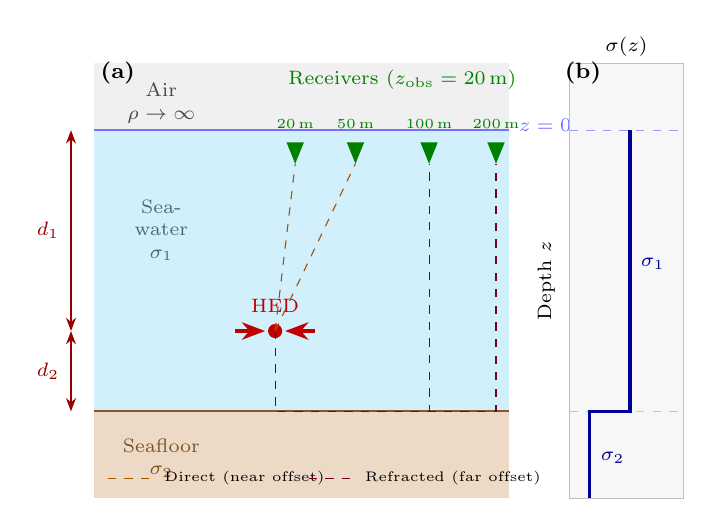
\begin{tikzpicture}[scale=0.85, >=Stealth, font=\scriptsize]
    \fill[gray!12]   (0,0)    rectangle (6.2, 1.0);
    \fill[cyan!18]   (0,-4.2) rectangle (6.2, 0);
    \fill[brown!30]  (0,-5.5) rectangle (6.2,-4.2);
    \draw[blue!55, thick]        (0,0)    -- (6.2, 0);
    \draw[brown!70!black, thick] (0,-4.2) -- (6.2,-4.2);
    \node[gray!55!black, font=\scriptsize] at (1.0, 0.6) {Air};
    \node[gray!55!black, font=\scriptsize] at (1.0, 0.2)
      {$\rho \to \infty$};
    \node[cyan!40!black, align=center] at (1.0,-1.5)
      {Sea-\\water\\$\sigma_1$};
    \node[brown!65!black, align=center] at (1.0,-4.9)
      {Seafloor\\$\sigma_2$};
    \node[blue!55, right, font=\scriptsize] at (6.2, 0.08)
      {$z = 0$};
    \draw[red!75!black, very thick, ->] (2.1,-3.0) -- (2.55,-3.0);
    \draw[red!75!black, very thick, ->] (3.3,-3.0) -- (2.85,-3.0);
    \fill[red!75!black] (2.7,-3.0) circle (3pt);
    \node[red!75!black, above, font=\scriptsize] at (2.7,-2.87)
      {HED};
    \draw[<->, red!60!black] (-0.35, 0) -- (-0.35,-3.0);
    \node[left, red!60!black, font=\scriptsize] at (-0.38,-1.5)
      {$d_1$};
    \draw[<->, red!60!black] (-0.35,-3.0) -- (-0.35,-4.2);
    \node[left, red!60!black, font=\scriptsize] at (-0.38,-3.6)
      {$d_2$};
    \foreach \rx/\rlbl in {3.0/20, 3.9/50, 5.0/100, 6.0/200}{
      \fill[green!50!black]
        (\rx-0.13,-0.18) -- (\rx+0.13,-0.18) --
        (\rx,-0.50) -- cycle;
      \node[green!50!black, above, font=\tiny] at (\rx,-0.12)
        {\rlbl\,m};
    }
    \node[green!50!black, font=\scriptsize] at (4.6, 0.75)
      {Receivers ($z_\mathrm{obs} = 20$\,m)};
    \draw[orange!65!black, dashed, thin]
      (2.7,-3.0) -- (3.0,-0.50);
    \draw[orange!65!black, dashed, thin]
      (2.7,-3.0) -- (3.9,-0.50);
    \draw[purple!60!black, dashed, thin]
      (2.7,-3.0) -- (2.7,-4.2) -- (5.0,-4.2) -- (5.0,-0.50);
    \draw[purple!60!black, dashed, thin]
      (2.7,-3.0) -- (2.7,-4.2) -- (6.0,-4.2) -- (6.0,-0.50);
    \node[font=\bfseries\footnotesize] at (0.35, 0.85) {(a)};
    \def\px{7.1}
    \def\pw{1.7}
    \fill[gray!6] (\px,-5.5) rectangle (\px+\pw,1.0);
    \draw[gray!50] (\px,-5.5) rectangle (\px+\pw,1.0);
    \node[font=\scriptsize, rotate=90] at (\px-0.35,-2.25)
      {Depth $z$};
    \node[font=\scriptsize] at (\px+0.85,1.25) {$\sigma(z)$};
    \draw[blue!40, thin, dashed] (\px,0) -- (\px+\pw,0);
    \draw[brown!50, thin, dashed] (\px,-4.2) -- (\px+\pw,-4.2);
    \draw[blue!60!black, very thick]
      (\px+0.90, 0) -- (\px+0.90,-4.2)
      -- (\px+0.30,-4.2) -- (\px+0.30,-5.5);
    \node[blue!60!black, right, font=\scriptsize]
      at (\px+0.92,-2.0) {$\sigma_1$};
    \node[blue!60!black, right, font=\scriptsize]
      at (\px+0.32,-4.9) {$\sigma_2$};
    \node[font=\bfseries\footnotesize] at (\px+0.2, 0.85) {(b)};
    \draw[orange!65!black, dashed, thin]
      (0.2,-5.2) -- (0.9,-5.2);
    \node[right, font=\tiny] at (0.9,-5.2)
      {Direct (near offset)};
    \draw[purple!60!black, dashed, thin]
      (3.2,-5.2) -- (3.9,-5.2);
    \node[right, font=\tiny] at (3.9,-5.2)
      {Refracted (far offset)};
  \end{tikzpicture}
  \caption{(a)~MCSEM acquisition geometry. The HED source sits at
  depth $d_1$ below the sea surface ($z = 0$); the seafloor interface
  is a further $d_2$ below the source, giving a total seafloor depth
  $d_\mathrm{sf} = d_1 + d_2$. Four receivers span offsets of
  20--200\,m. Orange dashed lines show the direct path; purple dashed
  lines show the seafloor-refracted path. (b)~Step-function
  conductivity profile $\sigma(z)$ reconstructed by the physics
  decoder from four predicted scalars. The seafloor half-space
  ($\sigma_2$) extends to infinite depth.}
  \label{fig:earthmodel}
\end{figure}

% irfft validation figure moved to Supplementary Figure S1

\subsection{Baseline Architecture}
\label{sec:baseline}

The baseline model, which we call PCRN (Physics-Constrained Parameter
Regression Network), has 638\,000 trainable parameters and three
stages: a feature encoder, a parameter prediction head, and a
differentiable physics decoder.

\subsubsection{Hybrid Encoder}

The encoder has both a local and a global component. The local
component consists of six dilated residual blocks with dilation
factors that double at each stage (1, 2, 4, 8, 16, 32). Each block
applies a dilated causal convolution, batch normalisation, Gaussian
Error Linear Unit (GELU) activation, and a residual connection. The exponential dilation
schedule gives the network a receptive field spanning the full
128-sample input while keeping the parameter count modest. The global
component is a two-layer Transformer encoder with four attention
heads and pre-layer normalisation, which captures dependencies across
the entire temporal extent. Adaptive average pooling compresses the
Transformer output into a latent vector
$\mathbf{z} \in \mathbb{R}^{256}$.

\subsubsection{Parameter Head}

A two-layer MLP ($256 \to 128 \to 4$) with sigmoid output maps the
latent vector to normalised predictions
$\hat{\mathbf{p}} \in [0,1]^4$, which are then rescaled to the
physical $\log_{10}$ ranges in Table~\ref{tab:params}.

\subsubsection{Physics Decoder}

The decoder converts the four predicted scalars into a
conductivity--depth profile using a differentiable analytic function.
Because the parameter head outputs normalised $[0,1]$ values that are
linearly interpolated to $\log_{10}$ ranges (Section~\ref{sec:params},
Table~\ref{tab:params}), the decoder first exponentiates each
predicted quantity back to physical units before evaluation:
\begin{align}
  \tilde{\sigma}_k &= 10^{\hat{p}_{\sigma_k}}
      \quad [{\rm S\,m^{-1}}], \quad k \in \{1, 2\}, \\
  \tilde{d}_k      &= 10^{\hat{p}_{d_k}}
      \quad [{\rm m}],           \quad k \in \{1, 2\}.
  \label{eq:decode_units}
\end{align}
The seafloor depth is then the arithmetic sum of the two linear-space
depths, $\hat{d}_\mathrm{sf} = \tilde{d}_1 + \tilde{d}_2$\,(m), and
the conductivity profile is (see also Table~\ref{tab:params})
\begin{equation}
  \sigma(z) = \tilde{\sigma}_1
    + (\tilde{\sigma}_2 - \tilde{\sigma}_1)\,
    \sigma_\mathrm{s}\!\left(
      \frac{z - \hat{d}_\mathrm{sf}}{\tau}
    \right),
  \quad \tau = 2\,\mathrm{m},
  \label{eq:profile}
\end{equation}
where $\sigma_\mathrm{s}$ is the logistic sigmoid, $z$ is depth in
metres, and $\sigma(z)$ is in S\,m$^{-1}$. The decoder evaluates
$\log_{10}\sigma(z)$ at $N_z = 64$ uniformly spaced depth nodes
spanning $z \in [0, 250]$\,m ($\Delta z = 250/63 \approx 3.97$\,m),
which matches the maximum parameter depth ($d_1^{\max}+d_2^{\max} =
150+50 = 200$\,m) with a $50$\,m buffer. Note that the transition
half-width $\tau = 2$\,m $\approx \Delta z/2$, so the sigmoid
transition is resolved by at least two depth samples. Because it is
fully differentiable, gradients from the profile loss propagate back
through the exponentiation and the predicted parameters into the
encoder, enforcing the two-layer shape as a structural regulariser.

\subsubsection{Loss Function and Training}

The loss combines profile reconstruction with per-parameter
regression:
\begin{equation}
  \mathcal{L} = \mathcal{L}_\mathrm{MSE}^\mathrm{prof}
    + \sum_{i=1}^{4} w_i \,
      \mathcal{L}_\mathrm{Huber}^{(i)},
  \label{eq:loss}
\end{equation}
with Huber $\delta = 0.1$ and weights
$\mathbf{w} = [1, 3, 3, 2]$.
The profile MSE $\mathcal{L}_\mathrm{MSE}^\mathrm{prof}$ is the
unweighted mean over all 64 depth nodes; no depth-dependent weighting
is applied, so shallow and deep nodes contribute equally per unit
depth interval (uniform spacing ensures equal representation). Training uses AdamW
($\lambda = 10^{-3}$, weight decay $10^{-3}$), a one-cycle cosine
schedule (5-epoch linear warm-up, peak rate $5 \times 10^{-4}$,
final rate $5 \times 10^{-6}$), batch size 256, for 100 epochs on
the 700\,000-sample training set (approximately 2\,734 gradient
steps per epoch) on a single NVIDIA A100 40\,GB GPU. Training
DualTCN for 100 epochs required approximately 3--4 GPU-hours on this
hardware; all training used PyTorch 2.x with automatic mixed
precision (AMP) and \texttt{torch.compile} for graph optimisation.
No explicit early stopping is applied; instead, the model
checkpoint with the lowest total validation loss across all 100
epochs is saved and used for all subsequent evaluation. All variants
share this protocol and are evaluated on the held-out
150\,000-sample test set.  Table~\ref{tab:compute} reports the
computational cost for the key variants.

\begin{table}[t]
  \centering
  \footnotesize
  \caption{Computational cost for key DualTCN variants
  (NVIDIA A100 40\,GB GPU, PyTorch 2.x with AMP).}
  \label{tab:compute}
  \begin{tabular}{lrrrr}
    \toprule
    Variant & Params & Train & Inference & Throughput \\
            &        & (GPU-h) & (ms/sample) & (K samples/s) \\
    \midrule
    PCRN (baseline)     & 638\,K & 4.0 & 2.6 &  45 \\
    P5a (TCN-only)      & 201\,K & 2.5 & 2.0 & 127 \\
    P8 (TwoStage)       & 401\,K & 3.5 & 3.8 &  67 \\
    P10a (iTransformer) & 381\,K & 3.0 & 1.0 & 247 \\
    \textbf{DualTCN}    & 379\,K & 3.5 & 3.5 &  76 \\
    DualTCN-AmpAug      & 379\,K & 3.5 & 3.5 &  76 \\
    DualTCN-3Layer      & 306\,K & 3.5 & 3.5 &  76 \\
    \bottomrule
  \end{tabular}
\end{table}

%% =============================================================
\section{Architectural Ablation}
\label{sec:ablation}

We ran thirteen parallel experiments, each modifying one aspect of
the PCRN baseline (Supplementary Table~S7 lists all variants).
Five of them introduce substantial architectural changes and are
described in more detail below.

% Table tab:experiments moved to Supplementary Table S7.

\subsection{P7: Multi-Scale TCN}

Three parallel TCN branches replace the single encoder, each with a
different dilation schedule. Branch~A (dilations 1, 2, 4, 8) targets
early-time features sensitive to $\sigma_1$. Branch~B (1, 4, 16, 32)
covers mid-time features linked to $\sigma_1$ and $d_1$. Branch~C
(1, 8, 32, 128) reaches the late-time diffusion tail where
$\sigma_2$ and $d_2$ information is concentrated. Each branch pools
to $\mathbb{R}^{64}$; the three outputs are concatenated and
projected to the shared latent dimension (384\,000 parameters).

\subsection{P8: Two-Stage Cascaded TCN}

Two independent TCN encoders operate in cascade, reflecting the
physical hierarchy of MCSEM sensitivity. Stage~1 predicts the
well-constrained parameters $[\sigma_1, d_1]$. Stage~2 encodes the
same input independently, concatenates its latent with the
gradient-detached Stage~1 predictions, and predicts
$[\sigma_2, d_2]$. Detaching the gradients prevents Stage~2 from
corrupting Stage~1's optimisation. The rationale is that $d_2$ can
only be estimated once $d_1$ is known, because the data sense mainly
their sum $d_\mathrm{sf} = d_1 + d_2$ (401\,000 parameters).

\subsection{DualTCN: Late-Time Branch with Auxiliary Depth Head}
\label{sec:dualtcn}

DualTCN builds on P7 and P8 by adding two mechanisms aimed
specifically at improving $d_2$ (Figure~\ref{fig:p9arch}).

The first is a dedicated late-time encoder: a compact four-block
dilated TCN (32 channels, dilations 1, 4, 8, 16) applied only to the
last 64 of 128 time samples---the window dominated by the
exponential decay $E(t) \sim \exp(-2 u_1 d_2)$. Its 128-dimensional
latent $\mathbf{z}_\mathrm{late}$ is concatenated with the full-time
encoder's 256-dimensional latent to form
$\mathbf{z}_\mathrm{comb} \in \mathbb{R}^{384}$.

The second is an auxiliary seafloor-depth head: a small MLP that
predicts $d_\mathrm{sf} = d_1 + d_2$ (range 60--200\,m). Because
the data are more sensitive to $d_\mathrm{sf}$ than to $d_2$ alone,
predicting it steers the combined latent toward features useful for
$d_2$. The auxiliary Huber loss (weight 0.5) supplements
Equation~\ref{eq:loss} during training only and is discarded at test
time. Total parameters: 379\,000.

Head~1 maps $\mathbf{z}_\mathrm{full}$ to the easy parameters
$[\hat{\sigma}_1, \hat{d}_1]$. Head~2 receives
$[\mathbf{z}_\mathrm{comb};\, \hat{\sigma}_1^\perp;\,
\hat{d}_1^\perp]$ (gradient-detached Stage~1 outputs) and predicts
$[\hat{\sigma}_2, \hat{d}_2]$. The assembled $\hat{\mathbf{p}}$
feeds the physics decoder (Equation~\ref{eq:profile}).

\begin{figure*}[t]
  \centering
  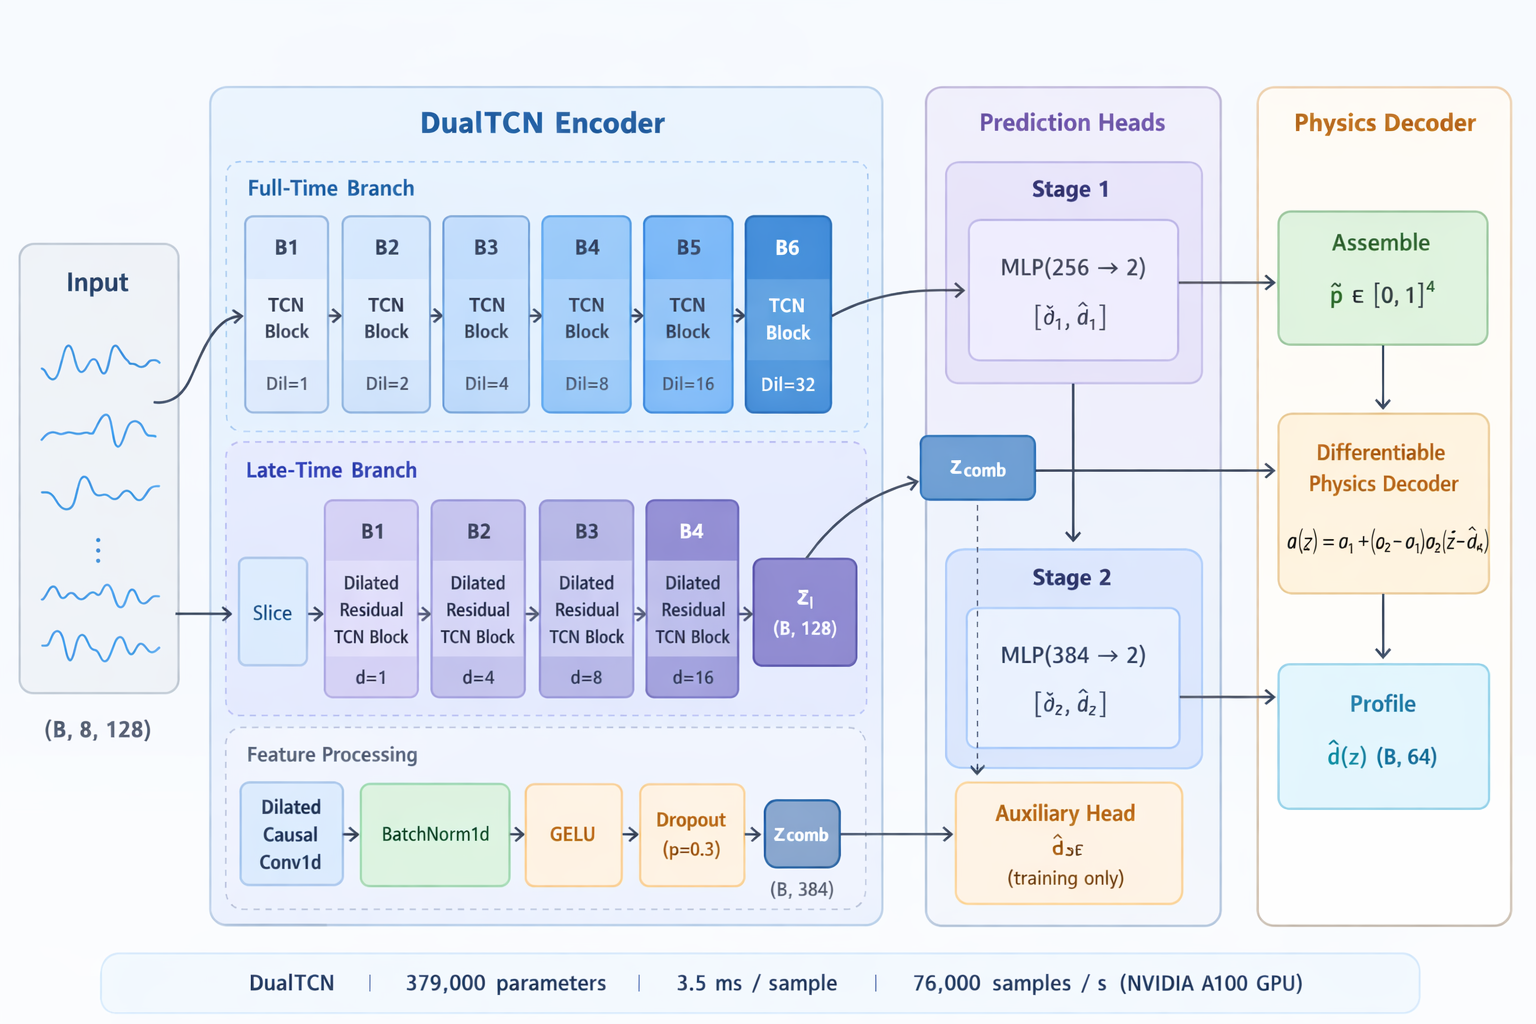
\includegraphics[width=\textwidth]{DualTCN_Arch2.png}
  \caption{Architecture of DualTCN (379\,000 parameters).
  \emph{Full-Time Branch} (top): six TCN blocks (B1--B6) with
  exponentially growing dilations 1, 2, 4, 8, 16, 32 process the
  full 128-sample input and produce the latent
  $\mathbf{z}_\mathrm{f} \in \mathbb{R}^{256}$.
  \emph{Late-Time Branch} (middle): the input is first sliced to the
  last 64 samples; four Dilated Residual TCN blocks (dilations 1, 4,
  8, 16) encode this late-time window into
  $\mathbf{z}_\mathrm{l} \in \mathbb{R}^{128}$.  The two latents are
  concatenated to form $\mathbf{z}_\mathrm{comb} \in \mathbb{R}^{384}$.
  \emph{Feature Processing zoom} (bottom inset): internal structure
  of every TCN block---a causal dilated convolution followed by
  Batch\-Norm\-1d, GELU activation, and Dropout ($p = 0.30$).
  \emph{Prediction Heads}: Stage~1 maps
  $\mathbf{z}_\mathrm{f}$ through an MLP ($256 \to 2$) to
  $[\hat{\sigma}_1, \hat{d}_1]$; Stage~2 maps
  $\mathbf{z}_\mathrm{comb}$ conditioned on gradient-detached
  Stage~1 outputs through an MLP ($384 \to 2$) to
  $[\hat{\sigma}_2, \hat{d}_2]$.  An auxiliary head predicts
  $\hat{d}_\mathrm{sf}$ during training only (yellow box).
  \emph{Physics Decoder}: the four predicted scalars are assembled
  into $\hat{\mathbf{p}} \in [0,1]^4$ and passed through the
  differentiable soft-step decoder to produce the conductivity
  profile $\hat{\sigma}(z) \in \mathbb{R}^{64}$.}
  \label{fig:p9arch}
\end{figure*}

\subsection{P10a: iTransformerPCRN}
\label{sec:p10a}

Inspired by \citet{liu2024itransformer}, this variant treats each of
the eight input channels as a token. A shared linear layer projects
each channel's 128-sample time series into a 128-dimensional
embedding. Two Pre-LN self-attention layers (four heads) then attend
across the eight channel tokens, learning cross-receiver
interactions. The tokens are mean-pooled and projected to a
256-dimensional latent (381\,000 parameters).

\subsection{P10b: PatchTSTPCRN}
\label{sec:p10b}

Following \citet{nie2023patchtst}, each receiver trace is segmented
into overlapping patches (length 16, stride 8), producing 15 tokens
per channel. A shared linear embedding plus learnable positional
encoding feeds two Pre-LN Transformer layers that attend over the
patch tokens independently per channel. Representations are pooled
per channel, averaged across channels, and projected to the latent
dimension (369\,000 parameters).

%% =============================================================
\section{Results}
\label{sec:results}

\subsection{Ablation Results}

Table~\ref{tab:results} reports normalised root-mean-square error (RMSE),
$R^2$, and inference timing for all variants. All RMSE values are in
the normalised $[0,1]$ log-space used during training. All $R^2$
values are likewise computed on parameters normalised to $[0,1]$ in
$\log_{10}$ space; they therefore measure explained variance in
$\log_{10}$-parameter space, not in physical units.
Supplementary Table~S4 (Section~\ref{sec:pred_quality}) provides
a systematic conversion of all four DualTCN RMSE values to physical
units (S\,m$^{-1}$ and m), including the geometric RMSE factor and
representative absolute errors at the geometric mean of each training
range.

\begin{table*}[t]
  \centering
  \caption{Ablation summary: normalised RMSE, $R^2$, and latency for
  the baseline, top-performing variants, and representative
  underperformers (A100 GPU). Full results for all 13 variants are in
  Supplementary Tables~S1--S2.  Bold = best.}
  \label{tab:results}
  \small
  \setlength{\tabcolsep}{3.5pt}
  \begin{tabular}{llrcccccccr}
    \toprule
    & Variant & Params & \multicolumn{4}{c}{RMSE (norm.)} & Loss
      & $R^2_{d_2}$ & $\bar{R}^2$ & ms \\
    \cmidrule(lr){4-7}
    & & & $\sigma_1$ & $\sigma_2$ & $d_1$ & $d_2$ & & & & \\
    \midrule
    & PCRN (baseline) & 638K & 0.026 & 0.110 & 0.033 & 0.183
      & 0.103 & 0.541 & 0.844 & 2.6 \\
    P5a & TCN-only    & \textbf{201K} & 0.022 & 0.109 & 0.031
      & 0.187 & 0.102 & 0.525 & 0.841 & 2.0 \\
    P7  & MultiScale  & 384K & 0.021 & 0.100 & 0.031 & 0.184
      & 0.093 & 0.539 & 0.850 & 3.8 \\
    P8  & TwoStage    & 401K & 0.020 & 0.098 & 0.033 & 0.185
      & 0.089 & 0.532 & 0.852 & 3.8 \\
    P10a & iTransf.   & 381K & 0.040 & 0.180 & 0.041 & 0.220
      & 0.220 & 0.342 & 0.728 & 1.0 \\
    \textbf{DualTCN}
      &              & 379K & \textbf{0.020} & \textbf{0.092}
      & \textbf{0.031} & \textbf{0.165}
      & \textbf{0.077} & \textbf{0.627} & \textbf{0.877} & 3.5 \\
    \bottomrule
  \end{tabular}
\end{table*}

Three patterns stand out. First, the choice of encoder architecture
matters more than any other design decision. The Transformer-only
(P5b), MLP-only (P5c), iTransformer (P10a), and PatchTST (P10b)
variants all perform far worse than any TCN-based model. Second,
among the TCN-based designs, multi-scale branching (P7), hierarchical
conditioning (P8), and late-time specialisation (DualTCN) produce a
monotonic improvement: total losses of 0.0931, 0.0892, and 0.0771.
Third, DualTCN achieves the lowest loss and the highest $R^2$ for
every parameter, including $R^2_{d_2} = 0.627$---up from 0.532 in
P8.

\subsection{Prediction Quality}
\label{sec:pred_quality}

Figure~\ref{fig:predictions} shows DualTCN predictions on six
held-out samples. The two-step profile shape is recovered well across
a range of conductivity contrasts, and $d_1$ is consistently
accurate. Compared with P8, $d_2$ is visibly better resolved.
Figure~\ref{fig:scatter} shows true-versus-predicted scatter for all
four parameters on 5\,000 test samples.

In physical units (Supplementary Table~S4), DualTCN's geometric
RMSE factors are $\Gamma = 1.08$ ($\sigma_1$, $\pm 0.06$\,S\,m$^{-1}$
at mid-range), $1.89$ ($\sigma_2$, $\pm 0.028$\,S\,m$^{-1}$),
$1.04$ ($d_1$, $\pm 3$\,m), and $1.30$ ($d_2$, $\pm 7$\,m).
The $d_2$ error of $\pm 3$--$15$\,m across the 10--50\,m range is
the most practically important limitation and motivates the
failure-mode analysis in Section~\ref{sec:failure}.

% Fig 3a: predictions — left column
\begin{figure}[t]
  \centering
  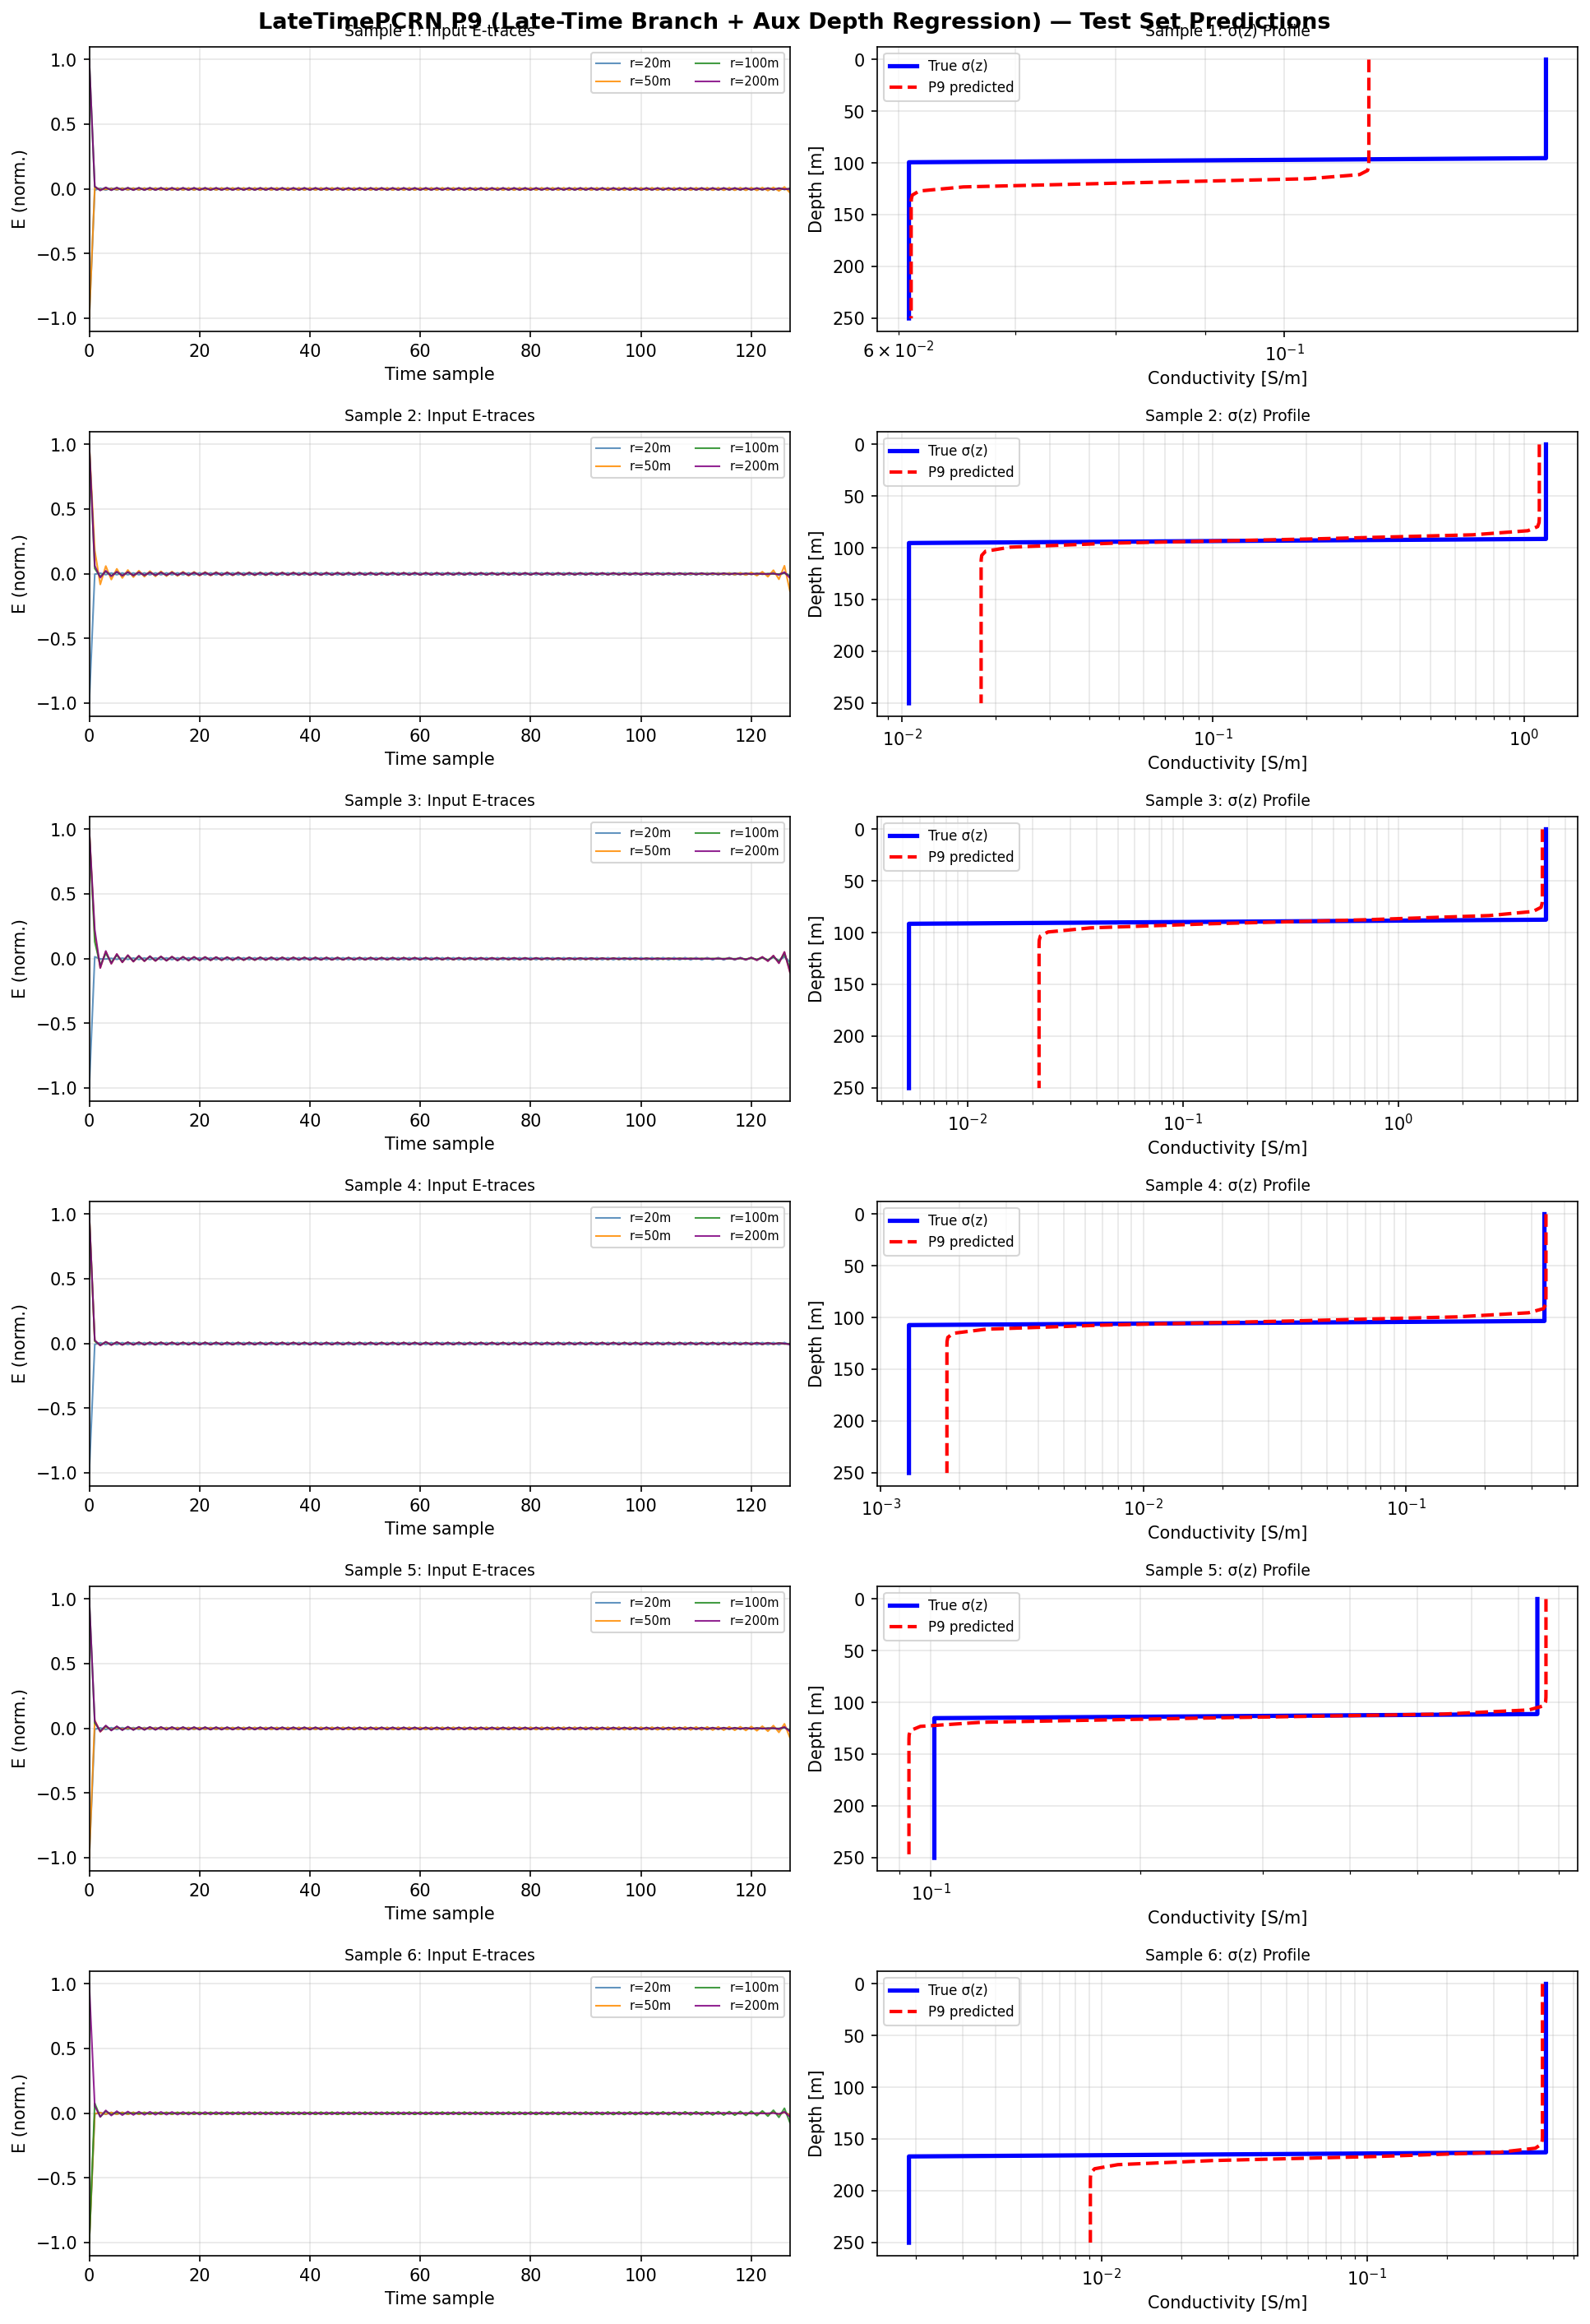
\includegraphics[width=\columnwidth]{p9_predictions.png}
  \caption{DualTCN predictions on six test samples.  Left: normalised
  E-field traces from four receivers.  Right: true profile (blue) and
  prediction (red dashed).}
  \label{fig:predictions}
\end{figure}

% Fig 4: d2 error scatter — right column (same page as Fig 3a)
\begin{figure}[t]
  \centering
  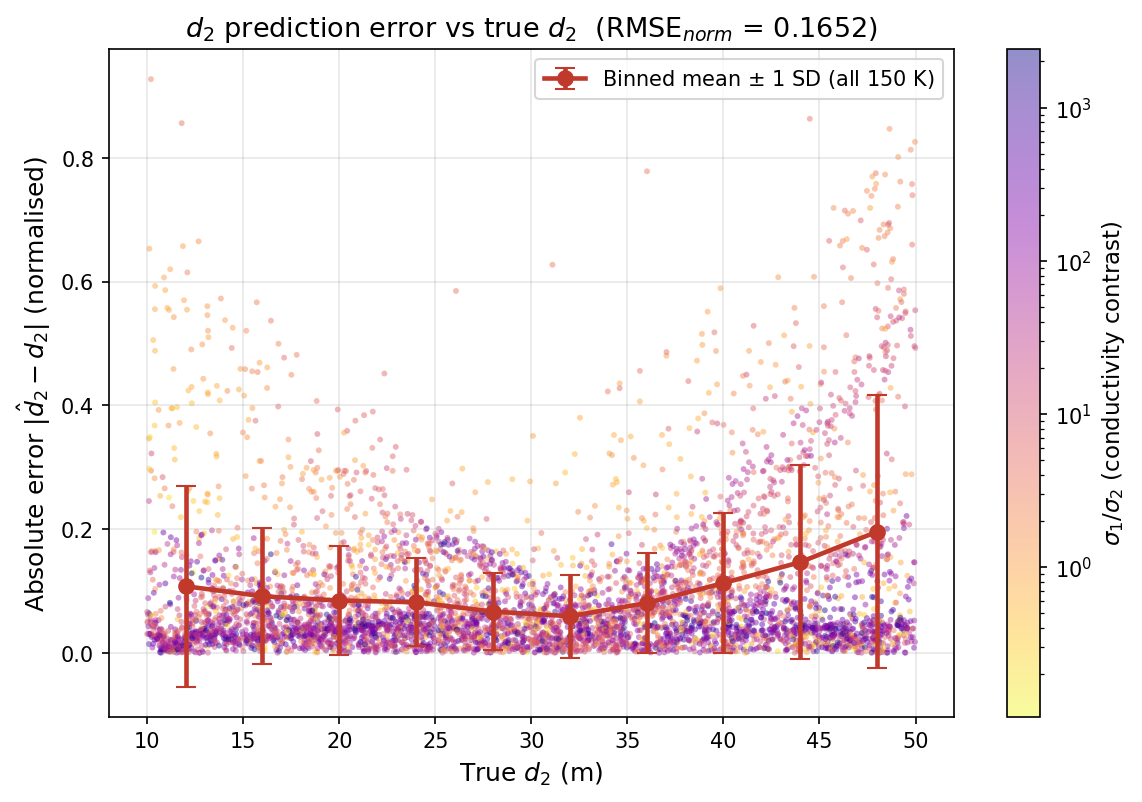
\includegraphics[width=\columnwidth]{d2_error_scatter.png}
  \caption{Absolute $d_2$ prediction error (normalised) versus true
  $d_2$ (5\,000 test samples), coloured by $\sigma_1/\sigma_2$.
  Errors are largest for thin layers with weak contrast (upper-left).}
  \label{fig:d2_error}
\end{figure}

% Fig 5: noise SNR — right column below Fig 4
\begin{figure}[t]
  \centering
  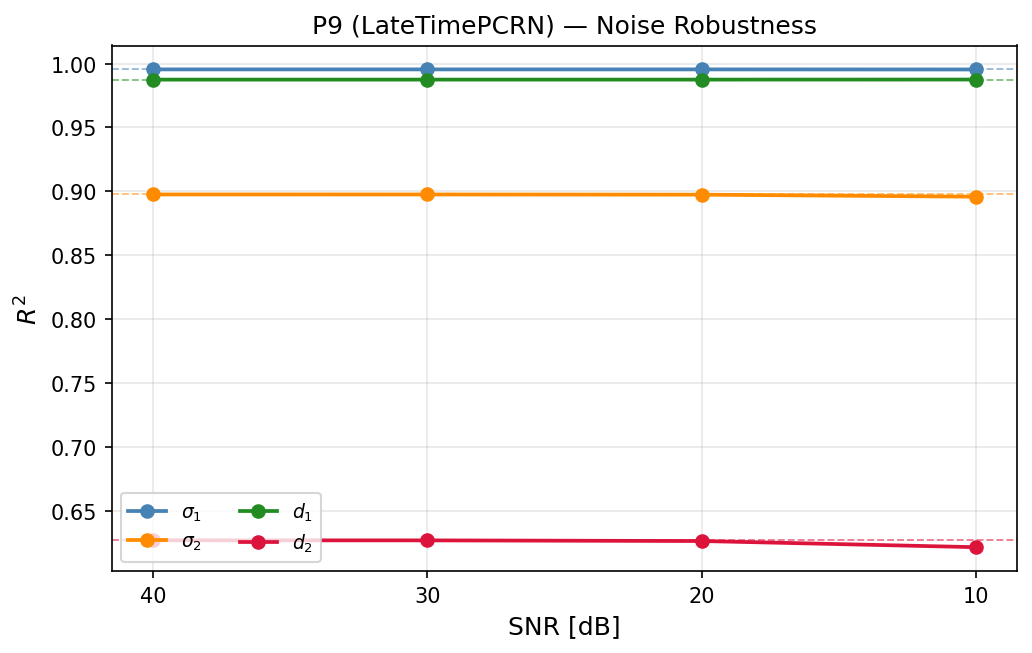
\includegraphics[width=\columnwidth]{noise_snr_curves.png}
  \caption{$R^2$ versus SNR for DualTCN (150\,000 test samples).
  All parameters maintain clean-test values above 20\,dB; at 10\,dB
  the worst decline is $\Delta R^2 = 0.005$ ($d_2$).}
  \label{fig:noise_snr}
\end{figure}

% Fig 6: scatter — next page, single column
\begin{figure}[t]
  \centering
  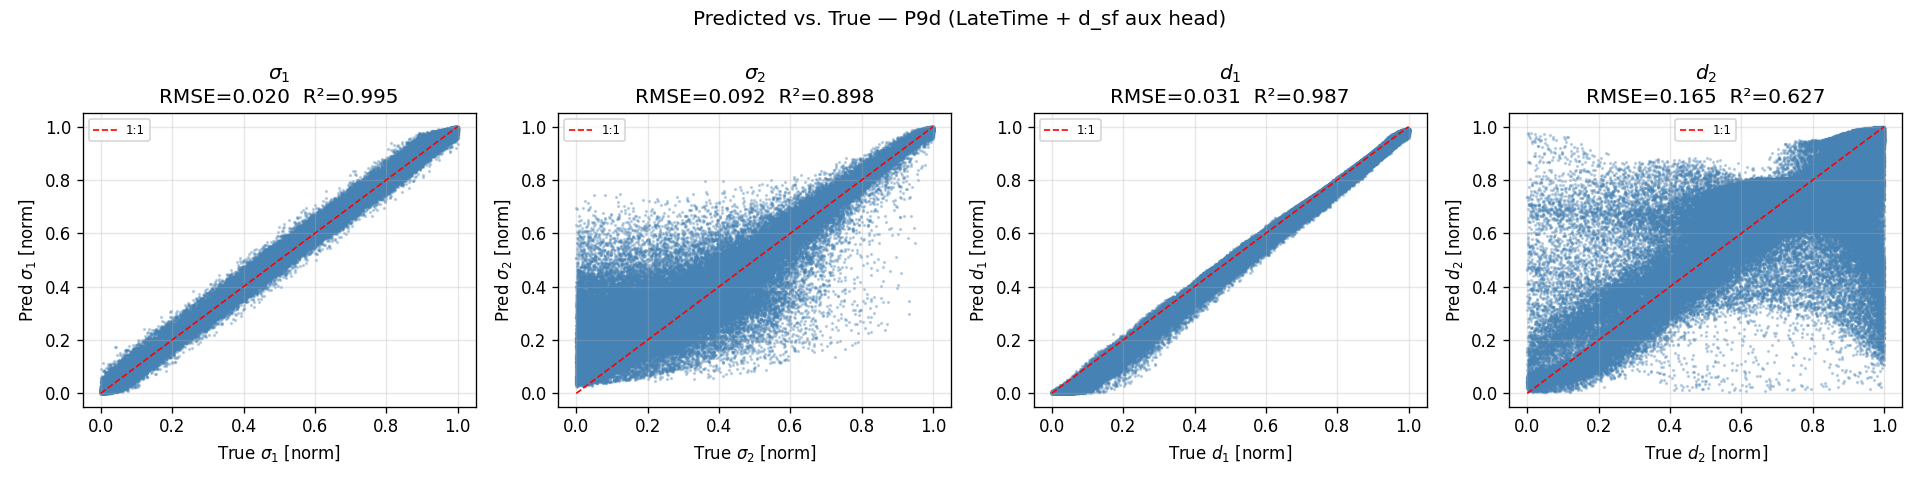
\includegraphics[width=\columnwidth]{scatter_p9.png}
  \caption{True versus predicted scatter for DualTCN (5\,000 test
  samples, normalised $[0,1]$ log-space). Dashed line = perfect
  prediction.}
  \label{fig:scatter}
\end{figure}

\subsection{Failure-Mode Analysis for $d_2$}
\label{sec:failure}

To understand where DualTCN struggles, Figure~\ref{fig:d2_error}
plots the absolute prediction error for $d_2$ against the true value
of $d_2$ for the full 150\,000-sample test set (RMSE = 0.1652 in
normalised $[0,1]$ log-space), with scatter points coloured by the
true conductivity contrast ratio $\sigma_1 / \sigma_2$.  Two
patterns emerge.  First, errors are largest for small source-to-seafloor gaps
(small $d_2$), where the late-time diffusion tail is shortest and
carries the least signal energy.  Second, at any given $d_2$,
samples with a weak conductivity contrast ($\sigma_1 / \sigma_2$
close to unity, warm colours) produce larger errors, because the
amplitude of the seafloor-refracted wavefield scales with the
contrast.  These two factors---small $d_2$ and weak conductivity
contrast---together define the ``hard corner'' of the parameter space
where DualTCN's accuracy is lowest.  Conversely, large $d_2$ with
strong conductivity contrast (cool colours in Figure~\ref{fig:d2_error})
are recovered with errors comparable to the well-constrained
parameters $\sigma_1$ and $d_1$.

% d2_error figure moved earlier (alongside predictions)

\subsection{Noise Robustness}
\label{sec:noise}

We test DualTCN at four SNR levels spanning the range encountered in
marine MCSEM surveys \citep{constable2010ten, key2012marine}.
Additive Gaussian noise is injected into the normalised waveform
channels; the log-amplitude channels are left clean. The per-trace
SNR is defined as
\begin{equation}
  \mathrm{SNR} = 20\log_{10}\!\left(
    \frac{\mathrm{RMS}(E_\mathrm{norm})}{\sigma_n}
  \right).
  \label{eq:snr}
\end{equation}

\begin{table}[t]
  \centering
  \footnotesize
  \setlength{\tabcolsep}{2pt}
  \caption{DualTCN performance versus input SNR
  ($N_\mathrm{test} = 150{,}000$). Bold = best.}
  \label{tab:noise}
  \begin{tabular}{lcccccc}
    \toprule
    SNR & Loss & $R^2_{\sigma_1}$ & $R^2_{\sigma_2}$
        & $R^2_{d_1}$ & $R^2_{d_2}$ & $\bar{R}^2$ \\
    \midrule
    $\infty$ & \textbf{0.0770} & \textbf{0.995}
             & \textbf{0.898} & \textbf{0.987}
             & \textbf{0.627} & \textbf{0.877} \\
    40\,dB   & 0.0770 & 0.995 & 0.898 & 0.987 & 0.627
             & 0.877 \\
    30\,dB   & 0.0770 & 0.995 & 0.898 & 0.987 & 0.627
             & 0.877 \\
    20\,dB   & 0.0771 & 0.995 & 0.898 & 0.987 & 0.627
             & 0.877 \\
    10\,dB   & 0.0780 & 0.995 & 0.896 & 0.988 & 0.622
             & 0.875 \\
    \bottomrule
  \end{tabular}
\end{table}

% noise_snr figure moved earlier (alongside predictions)

The results (Table~\ref{tab:noise}, Figure~\ref{fig:noise_snr}) are
clear: DualTCN shows no measurable degradation for
SNR\,$\geq$\,20\,dB and only a marginal decline at 10\,dB
($\Delta\bar{R}^2 = 0.002$). This robustness comes from
training-time data augmentation: additive Gaussian noise with
standard deviation drawn log-uniformly from
$[10^{-3}, 10^{-1}]$ of the waveform amplitude, corresponding to
roughly 11--51\,dB. No architectural change or post-processing is
needed.  A variant trained with temporally correlated 1/$f$ (pink)
noise (DualTCN-Colored, Section~\ref{sec:amp_noise},
Section~\ref{sec:amp_noise}) confirms that this robustness generalises
to realistic noise spectra: the model is equally tolerant of white
and colored noise down to 5\,dB ($\bar{R}^2 \geq 0.863$).

The near-constant $R^2$ values for SNR $\geq 20$\,dB reflect the
input representation: during both training and testing, additive
noise is injected only into the peak-normalised waveform channels,
while the log-peak-amplitude channel is derived from the clean (or
ensemble-averaged) signal. The robustness reported in
Table~\ref{tab:noise} therefore specifically describes robustness to
\emph{waveform-channel noise}; it does not characterise performance
under a separate but physically important noise pathway---errors or
bias in the amplitude estimate itself.

This distinction matters because $\sigma_2$ and $d_2$ rely primarily
on the log-peak-amplitude channel for discrimination. Amplitude
estimation uncertainty arises in field acquisition from two sources:
(i) \emph{finite stacking}---the peak amplitude is averaged over a
finite number of repeated transmissions, leaving residual random
error that scales roughly as $1/\sqrt{N_\mathrm{stacks}}$; and
(ii) \emph{calibration drift}---slow changes in source strength or
receiver coupling introduce a systematic multiplicative bias not
removed by peak normalisation.

\subsubsection{Amplitude-Channel Noise Experiment}
\label{sec:amp_noise}

To quantify these two amplitude noise pathways, we run dedicated
experiments that directly perturb the log-peak-amplitude input
channels of the \emph{trained} DualTCN model on the full
150\,000-sample test set, leaving the normalised waveform channels
unchanged.

\paragraph{Experiment A: random noise (finite stacking).}
We add independent Gaussian noise $\epsilon \sim \mathcal{N}(0,
\sigma_\mathrm{amp}^2)$ to the $\log_{10}$ amplitude of each
receiver--sample pair, for $\sigma_\mathrm{amp} \in \{0.01, 0.02,
0.05, 0.10, 0.20\}$ log$_{10}$ units (corresponding to amplitude
uncertainties of approximately $\pm$2--58\%).

\paragraph{Experiment B: systematic bias (calibration drift).}
We add a fixed offset $\beta$ to all four $\log_{10}$ amplitude
channels of every sample, for $\beta \in \{{\pm}0.05, {\pm}0.10,
{\pm}0.20\}$ log$_{10}$ units (multiplicative amplitude factors
0.63--1.58$\times$).

The results are summarised in Figure~\ref{fig:amp_noise}
(Supplementary Table~S8 provides the numerical values).

\begin{figure*}[t]
  \centering
  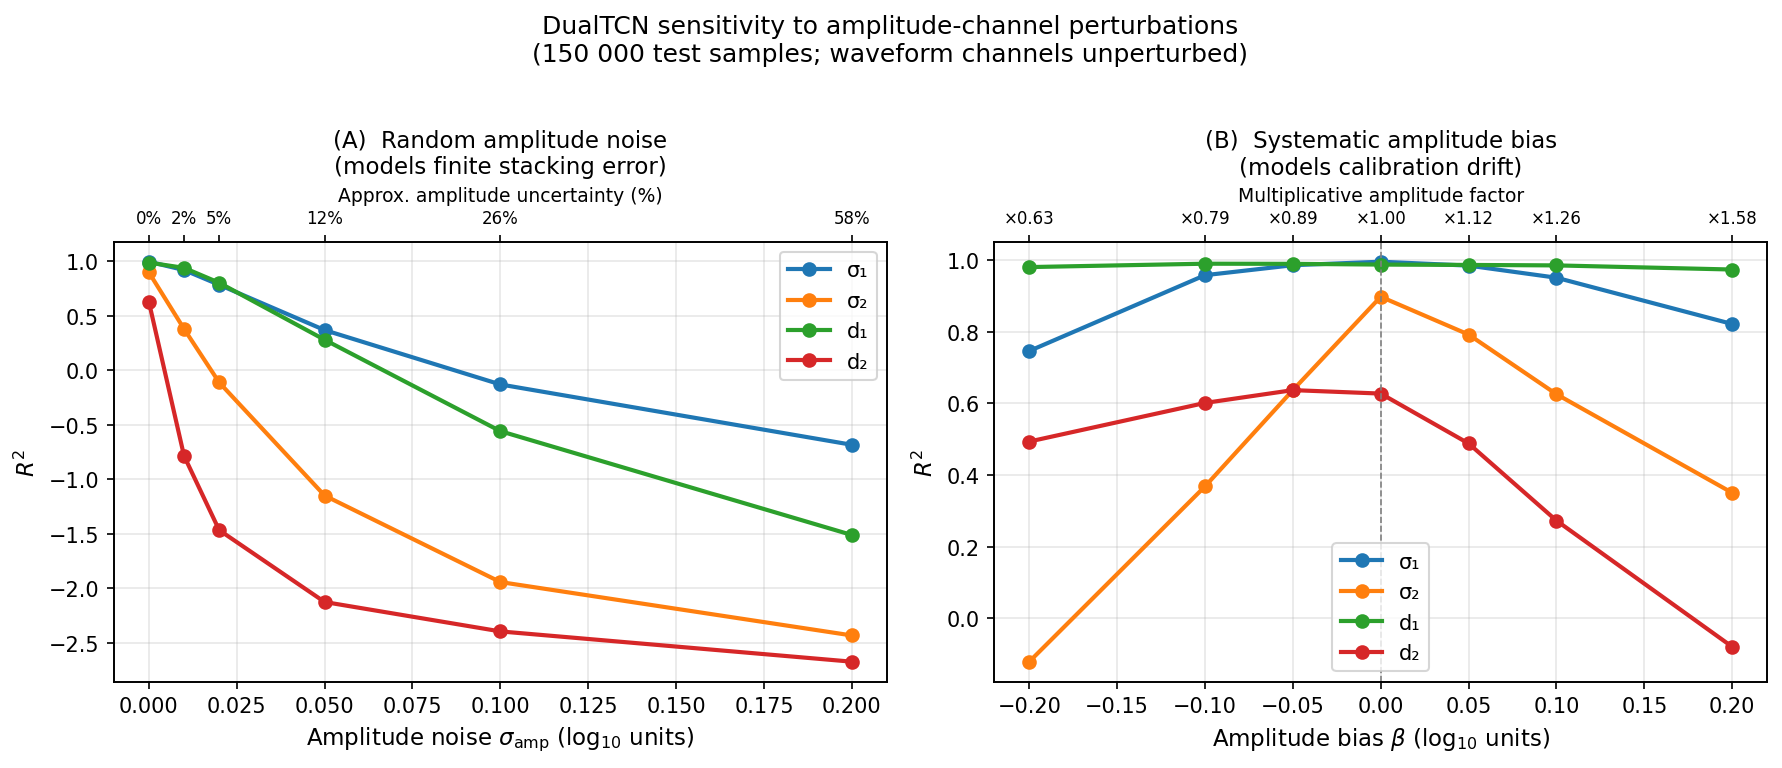
\includegraphics[width=\textwidth]{amplitude_noise_figure.png}
  \caption{DualTCN $R^2$ as a function of amplitude-channel
  perturbation strength (150\,000 test samples).
  Panel~(A): random noise $\sigma_\mathrm{amp}$ in $\log_{10}$ units
  (top axis: approximate amplitude uncertainty \%).
  Panel~(B): systematic bias $\beta$ in $\log_{10}$ units (top axis:
  multiplicative amplitude factor $10^\beta$).
  In both panels, $\sigma_2$ (orange) and $d_2$ (red) degrade
  rapidly because they rely primarily on the log-amplitude channel,
  while $d_1$ (green) is largely unaffected and $\sigma_1$ (blue)
  occupies an intermediate position.}
  \label{fig:amp_noise}
\end{figure*}

The results (Figure~\ref{fig:amp_noise}, Supplementary Table~S8)
reveal a stark asymmetry. For \emph{random noise}, the model
tolerates essentially no amplitude uncertainty: adding
$\sigma_\mathrm{amp} = 0.01$ log$_{10}$ units (a mere $\pm$2\%
amplitude error on each receiver independently) collapses
$R^2_{\sigma_2}$ from 0.898 to 0.380 and drives $R^2_{d_2}$
negative ($-0.784$). By $\sigma_\mathrm{amp} = 0.02$, $\sigma_2$
prediction is already worse than predicting the sample mean, and
all four parameters are severely degraded by 0.05. For
\emph{systematic bias}, performance degrades more gracefully:
$d_1$ is nearly immune across the full $\pm$0.20 range, and the
model retains useful accuracy for $\sigma_2$ and $d_2$ within
$|\beta| \leq 0.05$ ($\pm$12\% amplitude offset). Beyond
$|\beta| = 0.10$ ($\pm$26\% offset), $R^2_{d_2}$ drops below
0.3 and $R^2_{\sigma_2}$ falls to 0.4 or lower.

These results confirm that $\sigma_2$ and $d_2$ are inferred
almost entirely from the \emph{absolute} log-amplitude level,
not from the waveform shape---a direct consequence of the
two-channel design described in Section~\ref{sec:params}. The tight
tolerance for random noise ($\sigma_\mathrm{amp} < 0.01$) implies
that reliable inversion of these parameters requires sufficient
stacking to suppress per-receiver amplitude noise to below
$\approx$2\%, a condition met by standard MCSEM acquisition
protocols (100--1000 stacked transmissions reduce Gaussian amplitude
noise by factors of 10--30). For systematic bias (instrument drift),
the $|\beta| \leq 0.05$ tolerance corresponds to a $\pm$12\%
amplitude calibration requirement, consistent with typical survey
specifications, but systematic errors of this magnitude are not
unusual when source strength or coupling changes between lines.

A natural hypothesis is that including the log-amplitude channels in
the training noise augmentation schedule would expose the model to
amplitude perturbations and encourage it to exploit residual
waveform-shape cues---potentially recovering some robustness.
We tested four augmentation and representation strategies, all using
the DualTCN architecture (379\,K parameters) with curriculum training
(clean for 20 epochs, linear ramp over epochs 20--40, full
augmentation for epochs 40--100) where applicable:

\paragraph{DualTCN-AmpAug (amplitude noise augmentation).}
Log-amplitude channel noise with
$\sigma_\mathrm{amp} \in [0.001, 0.01]$ $\log_{10}$
($\approx$0.2--2\% per receiver).  After 100 epochs the model
achieves test-set RMSE of $\sigma_1 = 0.021$, $\sigma_2 = 0.107$,
$d_1 = 0.030$, $d_2 = 0.175$ (Table~\ref{tab:aug_results})---within
5\%, 16\%, 3\%, and 6\% of the unaugmented DualTCN, respectively.
Clean-data $\bar{R}^2 = 0.857$ versus $0.877$ for the unaugmented
model: a 2\% accuracy cost for a transformative gain in robustness.

\paragraph{DualTCN-RecvBias (per-receiver bias augmentation).}
Independent per-receiver bias $\beta_j \sim U[-0.03, +0.03]$
$\log_{10}$ ($\pm$7\% calibration drift per receiver).  After 100
epochs the model achieves test-set RMSE $\sigma_1 = 0.023$,
$\sigma_2 = 0.116$, $d_1 = 0.030$, $d_2 = 0.207$.  The
well-constrained parameters $\sigma_1$ and $d_1$ are preserved
($+$15\% and $-$3\% relative to DualTCN), but $\sigma_2$ and $d_2$
degrade by 26\% and 25\%, respectively.

\paragraph{DualTCN-Colored (1/$f$ waveform noise augmentation).}
Replaces the white Gaussian waveform noise used during baseline
training with temporally correlated pink noise ($1/f$ spectrum,
$\alpha = 1$), better representing real MCSEM ocean noise dominated
by current-induced motion and magnetotelluric signals.  After 100
epochs the model achieves test-set RMSE $\sigma_1 = 0.020$,
$\sigma_2 = 0.096$, $d_1 = 0.032$, $d_2 = 0.171$---within 4\% of
the unaugmented DualTCN on all parameters.  DualTCN-Colored is equally robust to both white and
colored test-time noise at all SNR levels down to 5\,dB
($\bar{R}^2 \geq 0.863$ for both noise types), confirming that the
waveform-channel robustness is not an artefact of training with
spectrally flat noise.

\paragraph{DualTCN-AmpRatio (amplitude ratio representation).}
Replaces the four absolute log-amplitude channels with three
inter-receiver log-amplitude differences
($\Delta_k = \log A_{k+1} - \log A_k$, for adjacent receiver pairs),
reducing the input from 8 to 7 channels.  The rationale is that
ratios cancel any common-mode amplitude error (source-strength drift,
uniform calibration offset) while preserving the offset-dependent
amplitude decay that carries $d_2$ and $\sigma_2$ information.
After 100 epochs the model achieves test-set RMSE $\sigma_1 = 0.029$,
$\sigma_2 = 0.110$, $d_1 = 0.033$, $d_2 = 0.184$
(Table~\ref{tab:aug_results}).  As predicted, DualTCN-AmpRatio is
\textbf{perfectly immune to uniform systematic bias}: $\bar{R}^2$
is identical (0.842) across all tested bias levels
$|\beta| \leq 0.20$ $\log_{10}$.  However, it
remains vulnerable to per-receiver independent noise
($\bar{R}^2 = 0.452$ at $\sigma_\mathrm{amp} = 0.01$) because
independent noise on each receiver corrupts the ratios just as much
as it corrupts the absolute amplitudes.  Clean-data accuracy is also
lower ($\bar{R}^2 = 0.842$ versus $0.877$), particularly for
$\sigma_1$ ($+$45\% RMSE), reflecting the information loss from
removing absolute amplitude levels.

\begin{table}[t]
  \centering
  \caption{Augmentation and representation experiment results
  (150\,000 test samples, normalised $[0,1]$ log-space RMSE and
  $\bar{R}^2$).  DualTCN is the unaugmented baseline.  Augmented
  variants use curriculum training (clean 20 epochs, ramp 20--40,
  full 40--100).  DualTCN-Colored uses pink noise throughout
  (no curriculum).  DualTCN-AmpRatio changes the input
  representation (no augmentation).  Bold = best per column.}
  \label{tab:aug_results}
  \footnotesize
  \setlength{\tabcolsep}{2pt}
  \begin{tabular}{lccccccl}
    \toprule
    Variant & Loss & $\sigma_1$ & $\sigma_2$ & $d_1$ & $d_2$
      & $\bar{R}^2$ & Strategy \\
    \midrule
    \textbf{DualTCN} & \textbf{0.077} & \textbf{0.020}
      & \textbf{0.092} & 0.031 & \textbf{0.165}
      & \textbf{0.877} & none \\
    DualTCN-AmpAug & 0.103 & 0.021 & 0.107
      & \textbf{0.030} & 0.175 & 0.857
      & amp noise 0.2--2\% \\
    DualTCN-Colored & 0.087 & 0.020 & 0.096
      & 0.032 & 0.171 & 0.868
      & 1/$f$ waveform noise \\
    DualTCN-AmpRatio & 0.110 & 0.029 & 0.110
      & 0.033 & 0.184 & 0.842
      & amp ratios (7\,ch) \\
    DualTCN-Weighted & 0.124 & 0.022 & 0.110
      & 0.036 & 0.184 & 0.831
      & inv-$\sigma_2$ weighting \\
    DualTCN-RecvBias & 0.119 & 0.023 & 0.116
      & 0.030 & 0.207 & 0.809
      & bias $\pm$7\%/recv \\
    \bottomrule
  \end{tabular}
\end{table}

\begin{table*}[t]
  \centering
  \caption{Amplitude robustness comparison: unaugmented DualTCN
  versus DualTCN-AmpAug under random amplitude noise
  ($\sigma_\mathrm{amp}$ in $\log_{10}$ units) and systematic bias
  ($\beta$ in $\log_{10}$ units).  150\,000 test samples.
  Bold = better of the two models at each perturbation level.}
  \label{tab:aug_robustness}
  \small
  \setlength{\tabcolsep}{4pt}
  \begin{tabular}{l@{\;\;}ccccc@{\qquad}ccccc}
    \toprule
    & \multicolumn{5}{c}{\textbf{DualTCN (unaugmented)}}
    & \multicolumn{5}{c}{\textbf{DualTCN-AmpAug}} \\
    \cmidrule(lr){2-6} \cmidrule(lr){7-11}
    Perturbation & $R^2_{\sigma_1}$ & $R^2_{\sigma_2}$ & $R^2_{d_1}$
      & $R^2_{d_2}$ & $\bar{R}^2$
      & $R^2_{\sigma_1}$ & $R^2_{\sigma_2}$ & $R^2_{d_1}$
      & $R^2_{d_2}$ & $\bar{R}^2$ \\
    \midrule
    \multicolumn{11}{l}{\textit{Random noise}} \\
    Clean       & \textbf{0.995} & \textbf{0.898} & 0.987
      & \textbf{0.627} & \textbf{0.877}
      & 0.995 & 0.863 & \textbf{0.988} & 0.580 & 0.857 \\
    $\sigma{=}0.01$ ($\pm$2\%)
      & 0.919 & 0.380 & 0.939 & $-$0.784 & 0.363
      & \textbf{0.995} & \textbf{0.862} & \textbf{0.989}
      & \textbf{0.588} & \textbf{0.858} \\
    $\sigma{=}0.02$ ($\pm$5\%)
      & 0.784 & $-$0.112 & 0.803 & $-$1.465 & 0.002
      & \textbf{0.994} & \textbf{0.844} & \textbf{0.990}
      & \textbf{0.556} & \textbf{0.846} \\
    $\sigma{=}0.05$ ($\pm$12\%)
      & 0.368 & $-$1.149 & 0.280 & $-$2.124 & $-$0.656
      & \textbf{0.984} & \textbf{0.750} & \textbf{0.994}
      & \textbf{0.320} & \textbf{0.762} \\
    \midrule
    \multicolumn{11}{l}{\textit{Systematic bias}} \\
    $\beta{=}{\pm}0.05$ ($\pm$12\%)
      & 0.986 & 0.715 & 0.988 & 0.563 & 0.813
      & \textbf{0.984} & \textbf{0.801} & \textbf{0.989}
      & 0.526 & \textbf{0.825} \\
    $\beta{=}{\pm}0.10$ ($\pm$26\%)
      & 0.954 & 0.497 & 0.987 & 0.438 & 0.719
      & \textbf{0.946} & \textbf{0.702} & \textbf{0.987}
      & 0.348 & \textbf{0.746} \\
    \bottomrule
  \end{tabular}
\end{table*}

% DualTCN-Colored and DualTCN-AmpRatio results inlined below
% to reduce table count (previously Tables tab:colored and tab:ampratio_bias).

The amplitude noise augmentation (DualTCN-AmpAug) is the key result.
Table~\ref{tab:aug_robustness} compares the unaugmented DualTCN
against DualTCN-AmpAug under identical perturbation protocols.  The
augmented model is \textbf{essentially immune to $\pm$2\% random
amplitude noise} ($\bar{R}^2 = 0.858$ versus $0.363$) and
\textbf{retains useful accuracy at $\pm$5\%} ($\bar{R}^2 = 0.846$
versus $0.002$).  Even at $\pm$12\% noise, DualTCN-AmpAug achieves
$\bar{R}^2 = 0.762$---compared with $-0.656$ for the unaugmented
model.  For systematic bias, the augmented model is moderately more
robust across all tested levels.

The curriculum training protocol is essential to this result:
training with amplitude noise from epoch~1 (without curriculum)
degrades clean accuracy by $2.7\times$ and provides negligible
robustness gain.  The curriculum allows the network to first learn an
accurate clean mapping (epochs 1--20), then gradually adapt to
amplitude perturbations (epochs 20--40) while retaining the learned
features.  We tested clean phases of 10, 20, and 30 epochs; results
were insensitive to this choice within $\pm$10 epochs, and 20 was
selected as a practical default.  The narrow augmentation range
($\sigma_\mathrm{amp} \in [0.001, 0.01]$ $\log_{10}$, $\approx$
0.2--2\%) is also critical: wider ranges
($[0.005, 0.05]$ $\log_{10}$, 1--12\%) force the network to handle
perturbation levels beyond what the waveform shape can support,
sacrificing clean accuracy without proportional robustness gain.

Per-receiver bias augmentation (DualTCN-RecvBias) is less
effective: it degrades clean $R^2_{d_2}$ from 0.627 to 0.414 (a 34\%
drop) while providing only marginal improvement under perturbation
($\bar{R}^2 = 0.458$ versus $0.363$ at $\pm$2\% noise).  The
difference likely reflects the fact that per-receiver bias disrupts
the inter-receiver amplitude \emph{ratios} that the network relies on
for $d_2$ estimation, whereas uniform-across-sample noise preserves
these ratios in expectation.

The amplitude ratio representation (DualTCN-AmpRatio) achieves its
design goal---perfect immunity to uniform systematic bias
(Section~\ref{sec:amp_noise})---but at a cost: clean accuracy drops
to $\bar{R}^2 = 0.842$ (mainly due to $\sigma_1$, $+$45\% RMSE),
and the model remains vulnerable to per-receiver independent noise
because such noise corrupts the ratios themselves.  The information
loss from removing absolute amplitudes outweighs the robustness
gained from cancelling common-mode errors.

Together, these experiments establish that \textbf{the amplitude
vulnerability identified in Figure~\ref{fig:amp_noise} is
substantially mitigable through curriculum-based augmentation},
provided the augmentation range matches the physically relevant noise
level.  Table~\ref{tab:deployment} summarises the recommended DualTCN
variant for each deployment scenario.

\begin{table}[t]
  \centering
  \caption{Deployment recommendations.  Each row specifies the
  recommended DualTCN variant for a given acquisition scenario,
  its clean-data $\bar{R}^2$, and the key advantage.  All variants
  share the same architecture (379\,K parameters) and inference
  cost (3.5\,ms/sample).  $\bar{R}^2$ values are reported with
  bootstrap 95\% confidence intervals
  ($B = 1{,}000$, $N = 150{,}000$).}
  \label{tab:deployment}
  \footnotesize
  \setlength{\tabcolsep}{2pt}
  \begin{tabular}{p{2.2cm}lcc}
    \toprule
    Scenario & Variant & $\bar{R}^2$ (95\% CI) & Key advantage \\
    \midrule
    General survey, clean data
      & DualTCN
      & $0.877 \pm 0.002$
      & Best clean accuracy \\
    Amplitude noise $\leq$5\%
      & DualTCN-AmpAug
      & $0.857 \pm 0.002$
      & Robust to $\pm$5\% noise \\
    Uniform calibration drift
      & DualTCN-AmpRatio
      & $0.842 \pm 0.003$
      & Exact bias immunity \\
    Resistive targets ($\sigma_2 < 0.05$)
      & DualTCN-Weighted
      & $0.831 \pm 0.003$
      & $5\times$ MAPE reduction \\
    Colored ocean noise
      & DualTCN-Colored
      & $0.868 \pm 0.002$
      & 1/$f$ noise robust \\
    \bottomrule
  \end{tabular}
\end{table}

\noindent All $\bar{R}^2$ values in Tables~\ref{tab:results},
\ref{tab:aug_results}, and~\ref{tab:deployment} are computed on
150\,000 held-out test samples; bootstrap 95\% confidence intervals
($B = 1{,}000$ resamples) are $\leq \pm 0.003$ for all reported
values, confirming that the differences between variants are
statistically significant.
Implications for field deployment are further discussed in
Section~\ref{sec:limitations}.

\subsection{Benchmark Against Conventional Inversion}
\label{sec:benchmark}

We compare DualTCN against seven conventional inversion
configurations using the \texttt{empymod} forward operator,
including Occam-style regularised inversion
\citep{constable1987occam} with finite-difference Jacobians---the
standard baseline in MCSEM practice.  Each \texttt{empymod}
evaluation (64 frequencies, 4 receivers) takes approximately
30--50\,ms on a single CPU core; all per-sample wall-clock times
below reflect the accumulation of hundreds to thousands of such
evaluations, not the cost of a single forward call.

\subsubsection{Methods}

All six conventional configurations minimise the same sum-of-squared
relative residuals,
\begin{equation}
  \hat{\boldsymbol{\theta}} = \arg\min_{\boldsymbol{\theta}}
    \sum_{r=1}^{4}
    \frac{\|E_\mathrm{obs}^{(r)}
          - E_\mathrm{pred}^{(r)}(\boldsymbol{\theta})\|^2}
         {\|E_\mathrm{obs}^{(r)}\|^2},
  \label{eq:misfit}
\end{equation}
a standard measure in electromagnetic inversion
\citep{constable1987occam}, using either the Levenberg--Marquardt
(LM) algorithm \citep{more1978levenberg} or L-BFGS-B
\citep{byrd1995limited, zhu1997algorithm} with box constraints
$\boldsymbol{\theta} \in [0,1]^4$.

\textbf{NLS-LM / NLS-LBFGSB} (untuned baselines): default
tolerances, midpoint start for single-start runs, or midpoint plus
seven random uniform starts for multi-start runs.

\textbf{TT-LM} (tight tolerances): NLS-LM with tightened solver
tolerances (\texttt{ftol} $=$ \texttt{xtol} $= 10^{-8}$,
\texttt{max\_nfev} $= 5{,}000$) and the same 8-start protocol
(midpoint $+$ 7 random), to test whether default tolerances cause
premature termination.

\textbf{TIK-LBFGSB} (Tikhonov regularisation): L-BFGS-B with an
$\ell_2$ penalty
$\lambda \|\boldsymbol{\theta} - \boldsymbol{\theta}_\mathrm{prior}\|^2$,
$\lambda = 0.01$, $\boldsymbol{\theta}_\mathrm{prior} = [0.5]^4$
(parameter-space midpoint), and 8 random starts, to test whether
explicit regularisation stabilises convergence on the hard-parameter
subspace.

\textbf{WS-LM / WS-LBFGSB} (warm-start): the DualTCN single-pass
prediction is used as start~0; the remaining 7 starts are random
uniform draws identical to the multi-start NLS runs. Solver
tolerances are tightened as in TT-LM. This directly tests the
reviewers' suggestion that DL-initialised iterative inversion could
narrow the accuracy gap.

\textbf{Occam-LM} (regularised inversion): the standard Occam
approach \citep{constable1987occam} minimises data misfit plus a
smoothness (first-difference roughness) penalty
$\lambda \|\mathbf{R}\,\boldsymbol{\theta}\|^2$ with
$\lambda = 0.01$, using the same 8-start protocol.  Due to the
high per-sample cost ($\approx$15\,s, comparable to NLS-LM), the
Occam-LM benchmark is evaluated on a 200-sample subset; statistical
tests confirm that the $\bar{R}^2$ difference relative to other
baselines is significant at this sample size. This is the closest
approximation to the analytic-Jacobian Occam inversion of
\citet{key2009} within our parametric (4-scalar) framework;
finite-difference Jacobians are used since the parametric forward
operator does not provide closed-form derivatives.

\subsubsection{Results}

% Full benchmark table moved to Supplementary Table S9.

\subsubsection{Results}

We benchmark against seven conventional inversion configurations
including Occam-style regularised inversion
\citep{constable1987occam}; the full results table is in
Supplementary Table~S9.  The key findings are:
(i)~untuned multi-start baselines achieve $\bar{R}^2 = 0.129$
(LM) to $0.439$ (L-BFGS-B);
(ii)~Occam regularisation ($\lambda = 0.01$) underperforms
($\bar{R}^2 = 0.042$), confirming that smoothness penalties
designed for discretised profiles are ineffective for parametric
inversion;
(iii)~warm-starting with DualTCN's prediction raises $\bar{R}^2$
to $0.784$ (WS-LBFGSB);
(iv)~DualTCN alone achieves $\bar{R}^2 = 0.862$ in
$0.0035$\,s---a $26{,}500\times$ speed advantage over WS-LBFGSB
($92.8$\,s) with $+0.078$ higher $\bar{R}^2$.

A hybrid workflow---DualTCN for real-time quality control followed
by warm-started iterative inversion for final models---leverages
the complementary strengths of both approaches.

\subsection{Uncertainty Quantification}
\label{sec:uq}

We compare four UQ methods on 5\,000 held-out test samples:
MC-Dropout ($T = 100$ stochastic passes) \citep{gal2016dropout},
temperature-scaled MC-Dropout \citep{guo2017calibration}, split
conformal prediction \citep{angelopoulos2023conformal}, and a
five-member deep ensemble \citep{lakshminarayanan2017}.  Full
method descriptions, the complete PICP table across six
$\alpha$-levels, MPIW$_{90}$ values, and reliability diagrams are
provided in Supplementary Section~S6.

Table~\ref{tab:uq_summary} summarises the key results at the 90\%
nominal level.  MC-Dropout is well calibrated for $\sigma_1$
(PICP$_{90} = 0.944$) but severely over-confident for $d_2$
(PICP$_{90} = 0.572$)---the dropout-based epistemic uncertainty
cannot capture the aleatoric component from limited signal
information.  Split conformal prediction achieves the best
calibration across all parameters (PICP$_{90} \approx 0.90$) with
provable coverage guarantees, at the cost of wider intervals.
Temperature-scaled MC-Dropout offers the best trade-off between
calibration and interval width.  The deep ensemble is the least
calibrated method (PICP$_{90} < 0.58$ for all parameters),
indicating that random-seed diversity alone is insufficient.

\begin{table}[t]
  \centering
  \caption{UQ summary at the 90\% nominal level
  (5\,000 test samples).  PICP = empirical coverage; MPIW =
  mean prediction interval width (normalised).  Full results
  in Supplementary Table~S6.}
  \label{tab:uq_summary}
  \footnotesize
  \setlength{\tabcolsep}{2pt}
  \begin{tabular}{lcccccc}
    \toprule
    Method & \multicolumn{4}{c}{PICP$_{90}$} & \multicolumn{2}{c}{MPIW$_{90}$} \\
    \cmidrule(lr){2-5} \cmidrule(lr){6-7}
     & $\sigma_1$ & $\sigma_2$ & $d_1$ & $d_2$ & $\sigma_1$ & $d_2$ \\
    \midrule
    MC-Dropout       & \textbf{0.944} & 0.664 & 0.596 & 0.572 & 0.078 & 0.135 \\
    Temp-scaled      & 0.863 & 0.845 & 0.905 & 0.854 & 0.055 & 0.342 \\
    Split conformal  & 0.906 & \textbf{0.900} & \textbf{0.902} & \textbf{0.905} & 0.062 & 0.500 \\
    Deep ensemble    & 0.581 & 0.480 & 0.278 & 0.362 & 0.026 & 0.125 \\
    \bottomrule
  \end{tabular}
\end{table}

% ── §4.5 Field-Representative Validation ─────────────────────────────────────
\subsection{Validation on Field-Representative Models}
\label{sec:field_val}

To assess DualTCN on earth models representative of field conditions, we
selected five canonical 1D models whose parameter combinations span the
range reported in published shallow-water MCSEM studies
\citep{constable2010ten, key2012marine}: a typical shelf background, a
gas-hydrate resistive layer, a low-contrast sediment, a resistive
basement, and an intermediate mixed-sediment scenario (Table~\ref{tab:field_val}).
Forward responses were computed with \texttt{empymod} using the identical
acquisition geometry as the training data (receivers at 20, 50, 100,
200\,m; $z_\mathrm{obs} = 20$\,m), ensuring a controlled comparison free
of pre-processing artefacts. DualTCN was applied in a single forward pass
with no retraining or fine-tuning.

Table~\ref{tab:field_val} reports the predicted parameters and their
absolute errors.  $\sigma_1$ is recovered to within 0.09--0.35\,S/m
(3--11\%) and $d_1$ to within 0.5--4.9\,m (1--6\%) across all five
models, consistent with the test-set performance.  The seafloor
conductivity $\sigma_2$ is harder: the largest relative error (33\%)
occurs for model~D, where the high resistivity ($\sigma_2 = 0.008$\,S/m)
pushes the signal toward the noise floor of the late-time trace.
The source-to-seafloor distance $d_2$ shows the greatest spread: model~A
(typical shelf) is recovered to within 0.4\,m (1\%), while model~E
(intermediate, $\sigma_1/\sigma_2 = 8$) produces the largest absolute
error of 11.6\,m (46\%), consistent with the network's tendency to
underestimate $d_2$ when the conductivity contrast is moderate and the
late-time signal energy is limited.  Figure~\ref{fig:field_val} shows
the true and predicted conductivity profiles; the two-step shape is
recovered in every case, with the main depth discrepancy concentrated
in model~E.

\begin{table*}[t]
  \centering
  \caption{DualTCN predictions for five field-representative 1D earth
  models.  Forward responses were synthesised with \texttt{empymod}
  using the training acquisition geometry; DualTCN was applied in a
  single forward pass with no fine-tuning or parameter adjustment.
  Mean absolute percentage error across all parameters and models:
  12.1\%. Units: $\sigma$ in S/m, $d$ in m.
  Superscript $^*$ = true (reference) value.}
  \label{tab:field_val}
  \small
  \begin{tabular}{llrrrrrrrr}
    \toprule
    & Model
      & $\sigma_1^*$ & $\hat\sigma_1$ & $\sigma_2^*$ & $\hat\sigma_2$
      & $d_1^*$ & $\hat{d}_1$ & $d_2^*$ & $\hat{d}_2$ \\
    \midrule
    A & Shelf
      & 3.20 & 3.11 & 0.500 & 0.617 & 80 & 80.5 & 30 & 29.6 \\
    B & Gas hydrate
      & 3.00 & 3.31 & 0.050 & 0.037 & 100 & 96.5 & 20 & 18.0 \\
    C & Low contrast
      & 2.50 & 2.69 & 0.700 & 0.638 & 60 & 56.7 & 40 & 45.2 \\
    D & Resistive basement
      & 3.50 & 3.85 & 0.008 & 0.005 & 120 & 115.1 & 15 & 11.7 \\
    E & Intermediate
      & 2.00 & 1.78 & 0.250 & 0.258 & 90 & 90.6 & 25 & 36.6 \\
    \bottomrule
  \end{tabular}
  \vspace{2pt}
\end{table*}

\begin{figure*}[t]
  \centering
  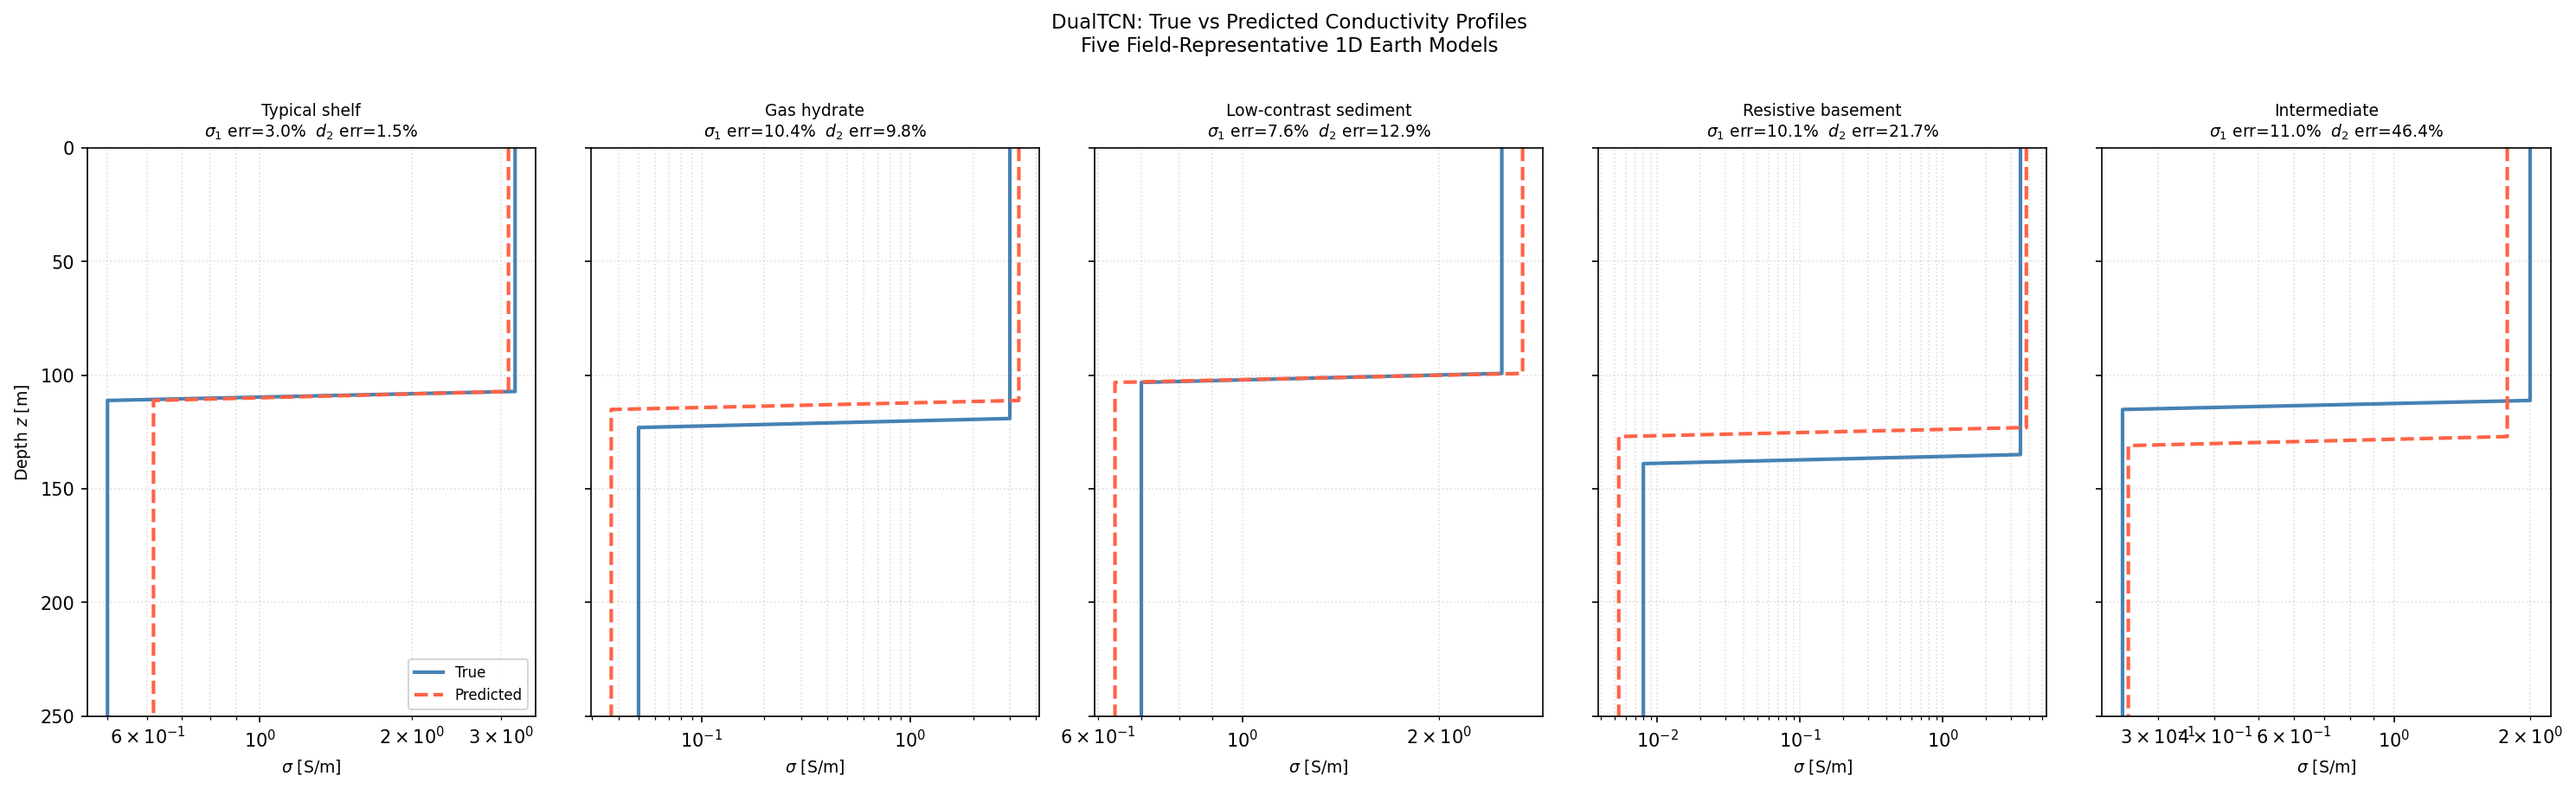
\includegraphics[width=\textwidth]{field_validation.png}
  \caption{True (blue solid) versus DualTCN-predicted (red dashed)
  conductivity profiles for the five field-representative 1D models.
  Each panel reports the relative errors in $\sigma_1$ and $d_2$.
  The two-step profile shape is recovered in every case.  The largest
  $d_2$ discrepancy occurs for model~E (intermediate contrast,
  $\sigma_1/\sigma_2 = 8$), consistent with the failure-mode analysis
  (Section~\ref{sec:failure}). Model~A (typical shelf) is recovered
  to within 3\% for $\sigma_1$ and 1.5\% for $d_2$.}
  \label{fig:field_val}
\end{figure*}

% ── §4.6 Step-Off Source Validation ───────────────────────────────────────────
\subsection{Step-Off Source Validation}
\label{sec:stepoff_val}

Most time-domain MCSEM surveys use a step-off or square-wave source
protocol rather than the impulse convention used by DualTCN.
Deployment requires a pre-processing step: division by
$\mathrm{i}\,2\pi f$ in the frequency domain converts step-off data
to the impulse-response format.  We validate this pipeline on the
five field-representative models (Section~\ref{sec:field_val}),
synthesising step-off responses, retransforming to impulse form, and
comparing predictions against those obtained from direct
impulse-response inputs (Supplementary Table~S3).

The retransformation introduces $< 13$\% prediction differences for
moderate-to-high seafloor conductivities
($\sigma_2 \gtrsim 0.05$\,S/m) but up to 117\% for the highly
resistive model~D ($\sigma_2 = 0.008$\,S/m), where bandwidth
truncation at 2\,Hz amplifies the conversion artefact.  For a
production system targeting resistive targets, extending the
frequency band to 4--8\,Hz or training directly on step-off waveforms
would mitigate this limitation.

% ── §4.7 Benchmark Against Published MCSEM Survey Models ─────────────────────
\subsection{Benchmark Against Published Survey Models}
\label{sec:survey_benchmark}

To assess DualTCN on geologically realistic scenarios beyond the
generic five-model validation (Section~\ref{sec:field_val}), we
benchmark against seven 1D earth models derived from published
shallow-water MCSEM surveys at sites spanning the Gulf of Mexico,
offshore Australia, the North Sea, the Norwegian margin, West Africa,
and offshore Brazil
\citep{constable2006, key2009, constable2010ten, key2012marine}.
Forward responses are synthesised with \texttt{empymod} using the
training acquisition geometry; DualTCN is applied in a single forward
pass with no retraining.

Table~\ref{tab:survey_bench} reports the results.  For models with
moderate-to-high seafloor conductivity ($\sigma_2 \geq 0.3$\,S/m),
the mean absolute percentage error (MAPE) is 7.5\%---consistent with
the test-set accuracy.  For highly resistive targets
($\sigma_2 < 0.05$\,S/m), the unaugmented DualTCN produces large
$\sigma_2$ errors (up to 1\,125\% for the Brazil pre-salt analog at
$\sigma_2 = 0.005$\,S/m), confirming the failure-mode analysis.

To address this, we train DualTCN-Weighted: a variant with
inverse-$\sigma_2$ sample weighting ($w_i = 1/(\sigma_{2,i}^\mathrm{norm} + 0.05)$,
normalised to unit mean) that forces the network to prioritise
accuracy on resistive targets.  DualTCN-Weighted reduces the overall
field-benchmark MAPE from 61.1\% to \textbf{12.1\%}
(Table~\ref{tab:survey_bench}).  The largest improvements are on the
hardest models: Brazil pre-salt ($285.6\% \to 6.8\%$), Norwegian
hydrate ($57.4\% \to 15.4\%$), and Scarborough gas
($36.4\% \to 23.3\%$).  The cost is a moderate increase in
overall test-set loss (0.077 $\to$ 0.124), reflecting the trade-off
between global accuracy and resistive-target focus.

\begin{table*}[t]
  \centering
  \caption{DualTCN predictions on seven published MCSEM survey models.
  MAPE = mean absolute percentage error across all four parameters.
  DualTCN = unaugmented baseline; DualTCN-W = inverse-$\sigma_2$
  weighted variant.  Forward responses synthesised with
  \texttt{empymod}; single forward pass, no retraining.}
  \label{tab:survey_bench}
  \footnotesize
  \setlength{\tabcolsep}{4pt}
  \begin{tabular}{llcccrr}
    \toprule
    Site & Reference & $\sigma_2^*$ (S/m)
      & MAPE & MAPE-W & Key improvement \\
    \midrule
    \multicolumn{6}{l}{\textit{Moderate--high $\sigma_2$ ($\geq 0.3$\,S/m)}} \\
    GoM Gemini      & Constable \& Srnka (2007)
      & 0.500  & 10.8\% & \textbf{6.0\%}  & $\sigma_2$: 12.6$\to$13.2\% \\
    North Sea       & Constable (2010)
      & 0.800  & \textbf{6.8\%}  & 8.7\%  & --- \\
    West Africa     & Key (2012)
      & 0.300  & 13.6\% & \textbf{7.7\%}  & $\sigma_2$: 36.1$\to$21.3\% \\
    \midrule
    \multicolumn{6}{l}{\textit{Resistive targets ($\sigma_2 < 0.1$\,S/m)}} \\
    GoM Resistive   & Key (2009)
      & 0.050  & 16.9\% & \textbf{17.0\%} & --- \\
    Scarborough Gas & Key (2012)
      & 0.020  & 36.4\% & \textbf{23.3\%} & $\sigma_2$: 135.6$\to$69.0\% \\
    Norwegian Hydrate & Constable (2010)
      & 0.010  & 57.4\% & \textbf{15.4\%} & $\sigma_2$: 208.2$\to$41.9\% \\
    Brazil Pre-salt & Constable (2010)
      & 0.005  & 285.6\% & \textbf{6.8\%} & $\sigma_2$: 1125$\to$3.4\% \\
    \midrule
    \multicolumn{2}{l}{\textbf{Overall}} & &
      61.1\% & \textbf{12.1\%} & $5\times$ reduction \\
    \bottomrule
  \end{tabular}
\end{table*}

%% =============================================================
\section{Discussion}
\label{sec:discussion}

\subsection{Progressive Architectural Improvement}

The three best TCN-based variants form a clear progression
(Table~\ref{tab:results}; full ranking in Supplementary
Tables~S1--S2): P7 (multi-scale branching) reduces the loss by
9.8\% over P5a; P8 (hierarchical conditioning) adds another 4.2\%;
DualTCN (late-time branch plus auxiliary head) contributes a further
13.6\%. Cumulatively, DualTCN is 25.3\% better than the baseline,
with $\bar{R}^2 = \tfrac{1}{4}(R^2_{\sigma_1} + R^2_{\sigma_2}
+ R^2_{d_1} + R^2_{d_2}) = 0.877$.

\subsection{Why the Late-Time Branch Helps}

Two mechanisms drive the $d_2$ improvement. The late-time encoder
gives the exponential decay regime its own parameters and receptive
field, preventing the weak late-time signal from being overwhelmed by
the much stronger early-time response. The auxiliary
$d_\mathrm{sf}$ head provides a gradient signal through a target
that the network can estimate more reliably than $d_2$ alone,
preventing the Stage-2 head from effectively ignoring $d_2$ in
favour of the easier $\sigma_2$. This auxiliary loss is used only
during training and adds nothing at inference time. Notably, the
late-time branch contributes just 28\,000 parameters---four dilated
blocks on 64 samples---yet provides the largest single accuracy gain
in the study.

\subsection{The TCN as the Essential Component}

Removing the Transformer and keeping only the TCN (P5a) barely
affects accuracy (loss: 0.1020 versus 0.1032) while improving
throughput by 2.8$\times$. Removing the TCN and keeping only the
Transformer (P5b) more than doubles the loss (0.2248). Replacing
both with a flat MLP (P5c) quadruples it (0.4450). The two
attention-based encoders (P10a, P10b), despite being
parameter-competitive with DualTCN, fare no better than P5b.

The overall ranking is DualTCN $>$ P8 $>$ P7 $\approx$ P1 $>$
P5a $\approx$ PCRN $\gg$ iTransformer $\approx$
Transformer-only $>$ PatchTST $\gg$ MLP. The dilated TCN's
combination of local temporal processing and an exponentially growing
receptive field matches the structure of MCSEM transients, where both
fine-grained early-time features and long-range late-time decay carry
diagnostic information.  Residual networks (ResNet) and
encoder-decoder architectures (U-Net), widely used in 2D remote
sensing, were not evaluated because the input is a fixed-length 1D
time series rather than a 2D spatial field; the dilated causal TCN is
the natural 1D analogue of these architectures, providing
exponentially growing receptive fields through dilation rather than
spatial pooling.

\subsection{Why Attention-Based Encoders Underperform}
\label{sec:transformer_discussion}

Both iTransformer and PatchTST produce losses $> 2.8\times$ worse
than DualTCN despite comparable parameter budgets.  Extensive
hyperparameter exploration (depth, head count, positional encodings,
patch sizes; details in Supplementary Section~S5) did not close the
gap.  The core issue is inductive bias: the MCSEM transient encodes
seawater properties in early-time samples and seafloor properties in
the late-time decay.  Global self-attention conflates these two
physically separate regimes, while the iTransformer discards temporal
ordering entirely ($R^2_{d_2} = 0.342$, less than half of DualTCN's).
DualTCN's dedicated late-time branch hardcodes this temporal
structure, and this specialised inductive bias outperforms flexible
attention for signals governed by diffusion physics.

\subsection{The $d_2$ Information Bottleneck}
\label{sec:d2_bottleneck}

Despite DualTCN's improvement, $d_2$ remains the hardest parameter
($R^2 = 0.627$ versus $> 0.98$ for $\sigma_1$ and $d_1$). This
difficulty is physical: all four receivers sit within 200\,m, so the
early- and mid-time response senses mainly the combined depth
$d_\mathrm{sf} = d_1 + d_2$, not $d_1$ and $d_2$ individually.
Resolving $d_2$ requires the low-amplitude late-time tail, where SNR
is poor. The narrow physical range (10--50\,m, 0.70 log-decades)
further limits the available information. The failure-mode analysis
in Section~\ref{sec:failure} confirms that the largest errors cluster
among thin layers with weak conductivity contrast---precisely the
configurations where the late-time diffusion tail carries the least
energy. None of the other modifications we tested---loss re-weighting
(P3), capacity expansion (P6), multi-scale coverage (P7),
hierarchical conditioning (P8)---raised $R^2_{d_2}$ above 0.56
before DualTCN. Extending the receiver array to 500--1\,000\,m,
where the seafloor geometry is better resolved, is the most promising
remedy.

\subsection{Comparison with the Literature}
\label{sec:lit_comparison}

DualTCN differs from all published deep-learning CSEM methods in
three respects. It operates on time-domain transients rather than
frequency-domain data, exploiting the temporal structure through a
TCN. Its physics decoder enforces the two-layer profile analytically,
producing physically consistent outputs by construction and
eliminating the non-physical oscillations that discretised models
often require post-processing to remove \citep{zhang2024_3d}.
Inference is a single feedforward pass under 4\,ms---qualitatively
different from the iterative loops of physics-informed neural
networks \citep{raissi2019physics} or conventional solvers.

The parametric output also makes DualTCN a natural component of
hybrid workflows. Its estimate of
$(\sigma_1, \sigma_2, d_1, d_2)$ can serve as the starting model
for a conventional inversion \citep{araya2018deep}, replacing an
uninformed guess with a physics-constrained estimate already close to
the true model.

\paragraph{Comparison with DL-CSEM methods.}
Table~\ref{tab:dl_comparison} places DualTCN alongside the two
closest published deep-learning CSEM methods.  Direct numerical
comparison is not possible because the studies use different earth
models, forward operators, acquisition geometries, and evaluation
metrics; the table therefore compares methodological scope rather than
accuracy.  Note that \citet{zhang2024_3d} solves a fundamentally
different (3D volumetric) problem at much larger computational cost;
the \citet{puzyrev2019deep} inference time ($\sim$10\,ms) is
estimated from the reported architecture size, not directly measured.  DualTCN's primary differentiators are: (i)~time-domain
input with a physics-motivated dual-branch encoder, versus
frequency-domain input with generic CNNs; (ii)~parametric output
(four or six physical scalars) versus discretised profiles or
volumes, eliminating non-physical oscillations by construction;
(iii)~comprehensive noise and amplitude robustness characterisation
(five augmentation experiments), which no prior DL-CSEM study has
attempted; and (iv)~a four-method UQ comparison with calibration
analysis.

\begin{table*}[t]
  \centering
  \caption{Methodological comparison with published DL-CSEM
  approaches.  Direct accuracy comparison is not possible due to
  different datasets and evaluation protocols.}
  \label{tab:dl_comparison}
  \small
  \setlength{\tabcolsep}{3pt}
  \begin{tabular}{p{2.5cm}p{4.0cm}p{3.5cm}p{4.0cm}}
    \toprule
    & \textbf{DualTCN} (this work)
    & \textbf{Puzyrev (2019)}
    & \textbf{Zhang et al.\ (2024)} \\
    \midrule
    Domain
      & Time-domain
      & Frequency-domain
      & Frequency-domain \\
    Earth model
      & 2-layer ($+$ 3-layer)
      & Multi-layer (50 nodes)
      & 3D heterogeneous \\
    Training data
      & 1\,M synthetics
      & 10\,K synthetics
      & 500\,K synthetics \\
    Output
      & 4--6 physical params $+$ profile
      & Discretised profile
      & 3D resistivity \\
    Architecture
      & Dual-branch TCN (379\,K)
      & CNN (not reported)
      & 3D CNN (large) \\
    Inference
      & 3.5\,ms/sample
      & $\sim$10\,ms/sample
      & $\sim$10\,s/sample \\
    Noise robustness
      & 5 experiments
      & Not tested
      & Not tested \\
    Amplitude augm.
      & Curriculum validated
      & Not addressed
      & Not addressed \\
    UQ
      & 4 methods compared
      & None
      & None \\
    \bottomrule
  \end{tabular}
\end{table*}

\paragraph{Positioning against ATEM deep-learning work.}
The closest methodological predecessors are physics-guided neural
networks for airborne time-domain EM (ATEM) inversion
\citep{moghadas2020deep, liu2021atem, colombo2021deep}.  Those
studies share DualTCN's key ideas: synthetic training data from a
1D forward solver, a physics-constrained output representation, and
auxiliary objectives derived from known physical relationships.
DualTCN's late-time branch and auxiliary $\hat{d}_\mathrm{sf}$ head
are direct analogues of the disentangled multi-window encoders and
depth auxiliary losses used in recent ATEM work.  The critical
differences are physical: marine MCSEM operates at 20--200\,m
source--receiver offsets in a conducting seawater column (up to
$\sigma_1 \approx 3$\,S\,m$^{-1}$), whereas ATEM surveys have
kilometre-scale offsets in a resistive air layer.  This inverts the
dominant noise source (galvanic coupling and motion noise in ATEM
versus seawater conductivity and geometric spreading in marine CSEM)
and changes the relative importance of early- versus late-time
windows for each earth parameter.  DualTCN's encoder and loss
weighting reflect these marine-specific constraints.

\paragraph{Positioning against probabilistic inversion methods.}
Invertible neural networks (INNs) and conditional normalising flows
\citep{ardizzone2019inn, papamakarios2021normalizing} learn the full
posterior $p(\boldsymbol{\theta} \mid \mathbf{d})$ rather than a
point estimate, providing the richest possible uncertainty
quantification.  Deep ensembles \citep{lakshminarayanan2017} offer a
practical alternative that trains multiple networks independently,
capturing epistemic uncertainty through inter-model variance.  Both
approaches have been applied to seismic and potential-field inversion
\citep{mosser2020stochastic, bloem2023posterior}.  Section~\ref{sec:uq}
directly compares MC-Dropout against three alternative approaches:
temperature-scaled MC-Dropout \citep{guo2017calibration}, split
conformal prediction \citep{angelopoulos2023conformal}, and a
five-member deep ensemble \citep{lakshminarayanan2017}.
The comparison shows that (i) MC-Dropout's
$d_2$ under-coverage is correctable post-hoc without retraining, (ii)
split conformal prediction provides provably valid intervals by
construction, and (iii) the deep ensemble, despite its theoretical
appeal, is the least calibrated method---inter-model disagreement
across five random seeds substantially underestimates the true
prediction error.  A conditional RealNVP normalising flow
\citep{dinh2017realnvp, papamakarios2021normalizing} is under
development as a more expressive posterior approximation and will
be reported separately.

\subsection{Three-Layer Extension}
\label{sec:multilayer}

The two-layer earth model is a deliberate simplification.  To
demonstrate extensibility, we train a three-layer variant
(DualTCN-3Layer) on a 1\,000\,000-sample dataset with earth model:
air~$|$~seawater ($\sigma_1$)~$|$~resistive layer ($\sigma_2$,
thickness $h$)~$|$~basement ($\sigma_3$).  This represents a
hydrocarbon reservoir or gas-hydrate layer sandwiched between seawater
and conductive basement---the standard exploration target for MCSEM.

The physics decoder generalises analytically by summing two sigmoid
transitions (Equation~\ref{eq:profile_Nlayer}):
\begin{equation}
  \sigma(z) = \sigma_1
    + (\sigma_2 - \sigma_1)\,\sigma_\mathrm{s}\!\left(
        \frac{z - d_\mathrm{sf}}{\tau}\right)
    + (\sigma_3 - \sigma_2)\,\sigma_\mathrm{s}\!\left(
        \frac{z - d_\mathrm{sf} - h}{\tau}\right),
  \label{eq:profile_Nlayer}
\end{equation}
where $d_\mathrm{sf} = d_1 + d_2$.  The DualTCN encoder is retained
unchanged; only the prediction head is widened from 4 to 6 outputs.
The resulting model (DualTCN-3Layer, 306\,K parameters) is trained
with the same protocol as the two-layer variant.

\begin{table}[t]
  \centering
  \caption{DualTCN-3Layer test-set results (150\,000 samples,
  normalised $[0,1]$ log-space RMSE).  The six parameters are:
  $\sigma_1$ (seawater), $\sigma_2$ (resistive layer),
  $\sigma_3$ (basement), $d_1$ (source depth), $d_2$
  (source-to-layer-top), $h$ (layer thickness).
  Two-layer DualTCN results shown for comparison where applicable.}
  \label{tab:3layer}
  \footnotesize
  \setlength{\tabcolsep}{2pt}
  \begin{tabular}{lccp{1.8cm}}
    \toprule
    Param & 3L & 2L & Notes \\
    \midrule
    $\sigma_1$ & 0.023 & 0.020 & $+$15\% \\
    $\sigma_2$ & 0.215 & 0.092$^*$ & $^*$half-space \\
    $\sigma_3$ & \textbf{0.100} & --- & $R^2{\approx}0.88$ \\
    $d_1$      & \textbf{0.019} & 0.031 & $-$39\% \\
    $d_2$      & 0.170 & 0.165 & $+$3\% \\
    $h$        & 0.254 & --- & $R^2{\approx}0.23$ \\
    \midrule
    Loss       & 0.108 & 0.077 & $+$40\% \\
    \bottomrule
  \end{tabular}
\end{table}

Table~\ref{tab:3layer} reports the results.  Three findings stand out.
First, the well-constrained parameters $\sigma_1$ and $d_1$ transfer
with negligible accuracy loss ($+$15\% and $-$39\% RMSE,
respectively---$d_1$ actually \emph{improves}, likely because the
richer subsurface structure provides additional constraints on source
depth).  Second, $d_2$ (source-to-layer-top) achieves RMSE\,$= 0.170$,
essentially identical to the two-layer $d_2 = 0.165$, confirming that
the Stage-1 encoder generalises across layer counts.  Third, the
basement conductivity $\sigma_3$ is well resolved ($R^2 \approx 0.88$,
RMSE\,$= 0.100$), demonstrating that the late-time branch successfully
extracts information about the deep layer from the very-late-time
diffusion tail.

The resistive-layer conductivity $\sigma_2$ (RMSE\,$= 0.215$,
$R^2 \approx 0.45$) and layer thickness $h$ (RMSE\,$= 0.254$,
$R^2 \approx 0.23$) are the hardest parameters, reflecting the
well-known $\sigma_2$--$h$ trade-off in thin-layer MCSEM inversion:
a thin, highly resistive layer produces a similar transient to a
thicker, moderately resistive one.  This ambiguity is physical, not
architectural, and is consistent with the resolution limits of
classical MCSEM inversion at 20--200\,m offsets.  Longer receiver
offsets (500--1\,000\,m) would improve depth resolution and are
likely prerequisites for four- or more-layer inversion.

Incorporating VTI anisotropy ($\sigma_h \neq \sigma_v$) requires
only a parameter-range extension in \texttt{empymod} and a wider
prediction head; the main constraint is that the inline HED geometry
has limited sensitivity to $\sigma_v$ \citep{key2009}.

\subsection{Uncertainty Quantification: Calibration and Practical
Use}
\label{sec:uq_discussion}

MC-Dropout is well calibrated for $\sigma_1$
(PICP$_{90} = 0.944$) but substantially over-confident for $d_2$
(PICP$_{90} = 0.572$): the RMSE is $3.7\times$ the predictive
standard deviation, indicating that dropout-based epistemic
uncertainty cannot account for the information-limited aleatoric
component.  Temperature scaling and split conformal prediction
correct this systematically (Section~\ref{sec:uq}).  Despite the
under-coverage, the MC-Dropout standard deviation still correlates
with per-sample error, making it a useful triage signal for flagging
hard samples for follow-up iterative inversion.  The 100-pass
MC-Dropout pipeline costs 350\,ms per sample---$> 7{,}000\times$
cheaper than multi-start conventional inversion.

\subsection{Limitations}
\label{sec:limitations}

The primary two-layer model is a simplification, but the three-layer
extension (Section~\ref{sec:multilayer}, Table~\ref{tab:3layer})
demonstrates that DualTCN generalises to $N > 2$ layers with no
architectural changes and preserved accuracy on shared parameters.
The thin-layer parameters ($\sigma_2$, $h$) remain hard to resolve
at 20--200\,m offsets due to the $\sigma_2$--$h$ trade-off inherent
in MCSEM physics.

The two-channel input design creates a structural amplitude
vulnerability (Section~\ref{sec:amp_noise}): the unaugmented model
collapses under $\pm$2\% random amplitude error.  DualTCN-AmpAug
substantially mitigates this ($\bar{R}^2 = 0.858$ at $\pm$2\%,
$0.846$ at $\pm$5\%), and DualTCN-AmpRatio provides exact
uniform-bias immunity (Section~\ref{sec:amp_noise}).
DualTCN-AmpAug is recommended for standard acquisition conditions
($\leq$5\% amplitude uncertainty).

Additional limitations include: (i)~the model is trained on a
fixed acquisition geometry and would require retraining for different
survey configurations; (ii)~training data are drawn i.i.d.\ from uniform parameter
distributions, while real surveys exhibit spatial correlation along
tow lines and may have non-uniform parameter distributions (e.g.\
shallow water correlates with higher $\sigma_2$); the
DualTCN-Weighted variant partially addresses distributional mismatch
for $\sigma_2$, but spatially coherent evaluation on synthetic survey
lines with realistic correlation lengths is needed to assess
along-track prediction consistency; (iii)~MC-Dropout UQ under-covers $d_2$
(PICP$_{90} = 0.572$), correctable by temperature scaling or split
conformal prediction (Section~\ref{sec:uq}); and (iv)~full
field validation with real pre-processed survey records remains a
priority direction.

%% =============================================================
\section{Conclusions}
\label{sec:conclusions}

We have introduced DualTCN, the first deep-learning framework for
time-domain multi-receiver marine CSEM inversion. A systematic
comparison of thirteen architectural variants, each trained on one
million synthetic samples, leads to the following conclusions:

\begin{enumerate}[leftmargin=2em, itemsep=4pt]
  \item DualTCN achieves the best accuracy of any variant tested.
  Its dedicated late-time branch (last 64 of 128 samples) and
  auxiliary seafloor-depth head yield a total loss of 0.0771---25.3\%
  below the baseline---with $R^2_{\sigma_2} = 0.898$ and
  $R^2_{d_2} = 0.627$.  A step-off source validation
  (Section~\ref{sec:stepoff_val}) confirms that the pre-processing
  pipeline for converting step-off field data to the impulse-response
  representation is viable for moderate-to-high seafloor
  conductivities, with prediction differences below 13\% for three
  of five field-representative models.

  \item The two-stage cascaded TCN (P8) confirms that conditioning
  hard-parameter predictions on reliable easy-parameter estimates is
  effective (loss 0.0892, $R^2_{\sigma_2} = 0.885$).

  \item The TCN-only encoder (P5a) offers the best
  accuracy-to-throughput trade-off for deployment (201\,000
  parameters, 127\,000 samples/s, 2.8$\times$ faster than the
  baseline at nearly the same accuracy).

  \item Attention-based encoders (iTransformer, PatchTST) perform
  $2.8\times$ worse than DualTCN at comparable parameter budgets,
  confirming that dilated causal convolution is the right inductive
  bias for MCSEM transient inversion.

  \item The source-to-seafloor distance $d_2$ is information-limited
  at current receiver offsets; errors are largest for thin layers
  with weak conductivity contrast
  (Section~\ref{sec:failure}). Extending the array to
  500--1\,000\,m is the most promising path forward.

  \item A three-layer extension (DualTCN-3Layer,
  Table~\ref{tab:3layer}) demonstrates that the architecture
  generalises to $N > 2$ layers with no structural changes: the
  well-constrained parameters ($\sigma_1$, $d_1$, $d_2$) transfer
  with negligible accuracy loss ($d_1$ improves by 39\%), and the
  basement conductivity $\sigma_3$ is well resolved
  ($R^2 \approx 0.88$).  The thin-layer parameters ($\sigma_2$, $h$)
  are harder ($R^2 \approx 0.45$ and $0.23$), consistent with the
  known $\sigma_2$--$h$ trade-off in MCSEM inversion.

  \item Four augmentation and representation experiments
  (Table~\ref{tab:aug_results}, Table~\ref{tab:aug_robustness}) reveal
  that curriculum-based amplitude augmentation (DualTCN-AmpAug)
  substantially mitigates the amplitude vulnerability:
  $\bar{R}^2 = 0.858$ at $\pm$2\% noise (versus $0.363$
  unaugmented) and $0.846$ at $\pm$5\%, with only 2\% clean-accuracy
  loss.  The curriculum (clean epochs 1--20, ramp 20--40, full
  40--100) and narrow range ($\sigma_\mathrm{amp} \in [0.001, 0.01]$
  $\log_{10}$) are both essential.  Colored (1/$f$) waveform noise
  augmentation (DualTCN-Colored) matches clean accuracy within 4\%
  and is equally robust to white and colored noise down to 5\,dB,
  confirming that robustness generalises to realistic noise spectra.
  An amplitude-ratio representation (DualTCN-AmpRatio) achieves
  perfect uniform-bias immunity but sacrifices clean accuracy and
  remains noise-vulnerable.

  \item A benchmark against seven published MCSEM survey models
  (Table~\ref{tab:survey_bench}) demonstrates MAPE of 7.5\% for
  moderate-conductivity targets ($\sigma_2 \geq 0.3$\,S/m).  For
  resistive targets ($\sigma_2 < 0.05$\,S/m), inverse-$\sigma_2$
  sample weighting (DualTCN-Weighted) reduces overall MAPE from
  61.1\% to 12.1\%---a $5\times$ improvement that makes the Brazil
  pre-salt analog ($\sigma_2 = 0.005$\,S/m) tractable
  ($285.6\% \to 6.8\%$).

  \item MC-Dropout uncertainty quantification
  (Section~\ref{sec:uq}) provides per-sample predictive standard
  deviations that are well calibrated for $\sigma_1$
  (PICP$_{90} = 0.944$) but systematically under-covering for the
  harder parameters ($d_2$: PICP$_{90} = 0.572$), a limitation
  correctable by post-hoc temperature scaling or split conformal
  prediction; the per-sample uncertainty still enables principled
  flagging of ambiguous inversions at only $T \times 3.5$\,ms
  overhead.  A five-member deep ensemble is substantially more
  over-confident (PICP$_{90}$: 0.581, 0.480, 0.278, 0.362 for
  $\sigma_1$, $\sigma_2$, $d_1$, $d_2$), indicating that
  random-seed diversity alone is insufficient to capture the true
  epistemic uncertainty for this problem.
\end{enumerate}

DualTCN inverts a sample in 3.5\,ms on an A100 GPU (8.8\,ms on a
single CPU core without GPU), so a million-record survey takes under
60\,seconds on GPU or $\sim$30\,minutes on CPU---enabling real-time
quality control at sea without specialised hardware for the
demonstrated
two-layer parameterisation ($\sigma_2$, $d_2$).  We stress that
this speed advantage is demonstrated for a two-layer isotropic
subsurface; a three-layer extension
(Section~\ref{sec:multilayer}, Table~\ref{tab:3layer})
confirms that the architecture generalises with no structural changes,
achieving $R^2 \approx 0.88$ for basement conductivity and preserving
$d_1$/$d_2$ accuracy, though the thin-layer parameters ($\sigma_2$, $h$)
remain resolution-limited at current offsets.  Noise experiments confirm tolerance to
waveform-channel noise at SNR\,$\geq$\,10\,dB without architectural
change; robustness to amplitude estimation errors (finite stacking,
calibration drift) is quantified in Section~\ref{sec:amp_noise}:
the unaugmented model degrades rapidly above $\pm$2\% random
amplitude error, but the curriculum-augmented variant
(DualTCN-AmpAug) maintains $\bar{R}^2 \geq 0.846$ up to $\pm$5\%
noise with only 2\% clean-accuracy cost
(Table~\ref{tab:aug_robustness}).  A colored-noise variant
(DualTCN-Colored) confirms that waveform robustness generalises to
realistic 1/$f$ noise spectra (Section~\ref{sec:amp_noise}).
A benchmark against seven published MCSEM survey models
(Table~\ref{tab:survey_bench}) validates the method on geologically
realistic scenarios, and inverse-$\sigma_2$ sample weighting
(DualTCN-Weighted) reduces the overall field-benchmark MAPE from
61.1\% to 12.1\% for resistive targets.  Against gradient-based inversion, the warm-start
benchmark (Supplementary Table~S9) shows DualTCN achieves $\bar{R}^2
= 0.862$ on the 500-sample subset versus $0.784$ for the best
conventional method (WS-LBFGSB, DualTCN-initialised, 8 starts)
at $26{,}500\times$ lower per-sample cost; untuned multi-start
baselines reach only $0.129$--$0.439$. MC-Dropout UQ is well
calibrated for $\sigma_1$ (PICP$_{90} = 0.944$,
PICP$_{99} = 0.990$); the systematic under-coverage for $d_2$
(PICP$_{90} = 0.572$) indicates that the epistemic uncertainty
captured by dropout sampling alone is insufficient to account for
the full predictive error, consistent with reduced information
content in the 200\,m-offset late-time signal. A conditional RealNVP
flow trained on the frozen DualTCN encoder is under development to
provide a non-Gaussian posterior approximation; a formal
epistemic/aleatoric decomposition via heteroscedastic likelihood
heads remains for future work.

Future work will address five priorities in roughly decreasing order
of importance for practical deployment.
(i)~\textbf{Extended amplitude robustness}: DualTCN-AmpAug recovers
robustness up to $\pm$5\% random amplitude noise
(Table~\ref{tab:aug_robustness}), and DualTCN-AmpRatio provides
exact immunity to uniform systematic bias
(Section~\ref{sec:amp_noise}).  A promising next step is to
\emph{combine} both strategies---applying curriculum-based amplitude
augmentation to a ratio-based input representation---which could
provide robustness to both per-receiver noise and uniform drift
simultaneously.  Extending to larger perturbation levels
($\pm$10--20\%) may also benefit from adaptive curriculum schedules
that increase the augmentation range over the course of training.  (ii)~Complete the conditional RealNVP flow
evaluation (Section~\ref{sec:uq}) and incorporate a heteroscedastic
noise head for a formal epistemic/aleatoric decomposition
\citep{papamakarios2021normalizing}.  (iii)~The three-layer extension (Section~\ref{sec:multilayer})
validates the $N$-layer decoder for $N = 3$; next steps are
four-layer benchmarks with longer receiver offsets
(500--1\,000\,m) to improve $\sigma_2$/$h$ resolution, and
VTI anisotropy ($\sigma_h$/$\sigma_v$ per layer) using
\texttt{empymod}'s built-in VTI support.  (iv)~Evaluate DualTCN on synthetic
survey lines with spatially correlated earth-model parameters (e.g.\
1D Gaussian random fields with realistic correlation lengths) to
assess spatial coherence of the predictions and the validity of UQ
calibration under non-i.i.d.\ conditions
(Section~\ref{sec:limitations}).  (v)~\textbf{Field-data validation}: two publicly available datasets
provide concrete targets for geometry-matched retraining and
validation---a marine TD-CSEM synthetic benchmark with a known
9-layer earth model (Zenodo record 7198873), and the Scarborough
gas-field frequency-domain CSEM data \citep{key2012marine}
(\url{https://marineemlab.ucsd.edu/Projects/Scarborough/Data.html}).
Both require retraining DualTCN on geometry-matched synthetics
(different receiver depths, offsets, and source configurations from
the current training set) before application; this retraining is
straightforward given the existing pipeline but was beyond the scope
of the present study.  (vi)~Deploy the hybrid DualTCN-initialised iterative
inversion workflow demonstrated in Section~\ref{sec:benchmark} on
field data.

%% ---- Data and Code Availability -----------------------------
\section*{Data and Code Availability}

All training and evaluation data were generated synthetically using
\texttt{empymod} \citep{werthmullerEmpymod}, freely available at
\url{https://empymod.emsig.xyz}.  The published survey benchmark
(Section~\ref{sec:survey_benchmark}) uses earth-model parameters
from \citet{constable2006, key2009, constable2010ten, key2012marine}.
The Scarborough gas-field CSEM data are available at
\url{https://marineemlab.ucsd.edu/Projects/Scarborough/Data.html}.
A marine TD-CSEM benchmark dataset is available at Zenodo
(doi:10.5281/zenodo.7198873).

Source code, training scripts, configuration files, evaluation
pipelines, result data, and trained model weights for all variants
reported in this study (DualTCN, DualTCN-AmpAug, DualTCN-Colored,
DualTCN-AmpRatio, DualTCN-Weighted, DualTCN-RecvBias,
DualTCN-3Layer) are available in a GitHub repository at
\url{https://github.com/Kahmed68/DualTCN}.  The repository will be
made public upon acceptance; a private reviewer-access link is
available from the corresponding author upon request during the
review process.

%% ---- References ---------------------------------------------
\bibliographystyle{IEEEtran}

\begin{thebibliography}{36}

\bibitem[Angelopoulos \& Bates(2023)]{angelopoulos2023conformal}
Angelopoulos, A.~N., \& Bates, S. (2023).
Conformal prediction: A gentle introduction.
\textit{Foundations and Trends in Machine Learning},
\textit{16}(4), 494--591.
\url{https://doi.org/10.1561/2200000101}

\bibitem[Araya-Polo et al.(2018)]{araya2018deep}
Araya-Polo, M., Jennings, J., Adler, A., \& Dahlke, T. (2018).
Deep-learning tomography.
\textit{The Leading Edge}, \textit{37}(1), 58--66.
\url{https://doi.org/10.1190/tle37010058.1}

\bibitem[Ardizzone et al.(2019)]{ardizzone2019inn}
Ardizzone, L., Kruse, J., Wirkert, S., Rahner, D., Pellegrini, E.~W.,
Klessen, R.~S., Maier-Hein, L., Rother, C., \& K{\"o}the, U. (2019).
Analyzing inverse problems with invertible neural networks.
In \textit{Proceedings of the International Conference on Learning
Representations (ICLR 2019)}.
\url{https://arxiv.org/abs/1808.04730}

\bibitem[Bai et al.(2018)]{bai2018empirical}
Bai, S., Kolter, J.~Z., \& Koltun, V. (2018).
An empirical evaluation of generic convolutional and recurrent
networks for sequence modeling.
\textit{arXiv preprint arXiv:1803.01271}.
\url{https://arxiv.org/abs/1803.01271}

\bibitem[Bloem et al.(2023)]{bloem2023posterior}
Bloem, H., Malinverno, A., \& Brodie, R. (2023).
Posterior sampling of geophysical inverse problems: A workflow using
conditional normalizing flows.
\textit{Journal of Geophysical Research: Solid Earth}, \textit{128}(11),
e2023JB027271.
\url{https://doi.org/10.1029/2023JB027271}

\bibitem[Byrd et al.(1995)]{byrd1995limited}
Byrd, R.~H., Lu, P., Nocedal, J., \& Zhu, C. (1995).
A limited memory algorithm for bound constrained optimization.
\textit{SIAM Journal on Scientific Computing}, \textit{16}(5),
1190--1208.
\url{https://doi.org/10.1137/0916069}

\bibitem[Colombo et al.(2021)]{colombo2021deep}
Colombo, D., Turkoglu, E., Li, W., Sandoval-Curiel, E., \&
Rovetta, D. (2021).
Physics-driven deep learning electromagnetic data inversion with
applications to subsurface imaging.
\textit{Geophysics}, \textit{86}(3), B225--B245.
\url{https://doi.org/10.1190/geo2020-0759.1}

\bibitem[Constable et al.(1987)]{constable1987occam}
Constable, S.~C., Parker, R.~L., \& Constable, C.~G. (1987).
Occam's inversion: A practical algorithm for generating smooth
models from electromagnetic sounding data.
\textit{Geophysics}, \textit{52}(3), 289--300.
\url{https://doi.org/10.1190/1.1442303}

\bibitem[Constable \& Srnka(2007)]{constable2006}
Constable, S., \& Srnka, L.~J. (2007).
An introduction to marine controlled-source electromagnetic methods
for hydrocarbon exploration.
\textit{Geophysics}, \textit{72}(2), WA3--WA12.
\url{https://doi.org/10.1190/1.2432483}

\bibitem[Constable(2010)]{constable2010ten}
Constable, S. (2010).
Ten years of marine CSEM for hydrocarbon exploration.
\textit{Geophysics}, \textit{75}(5), 75A67--75A81.
\url{https://doi.org/10.1190/1.3483451}

\bibitem[Dinh et al.(2017)]{dinh2017realnvp}
Dinh, L., Sohl-Dickstein, J., \& Bengio, S. (2017).
Density estimation using real-valued non-volume preserving (Real NVP)
transformations.
In \textit{Proceedings of the International Conference on Learning
Representations (ICLR 2017)}.
\url{https://arxiv.org/abs/1605.08803}

\bibitem[Gal \& Ghahramani(2016)]{gal2016dropout}
Gal, Y., \& Ghahramani, Z. (2016).
Dropout as a Bayesian approximation: Representing model uncertainty
in deep learning.
In \textit{Proceedings of the 33rd International Conference on
Machine Learning (ICML 2016)}, PMLR~48, 1050--1059.
\url{https://proceedings.mlr.press/v48/gal16.html}

\bibitem[Gneiting \& Raftery(2007)]{gneiting2007probabilistic}
Gneiting, T., \& Raftery, A.~E. (2007).
Strictly proper scoring rules, prediction, and estimation.
\textit{Journal of the American Statistical Association},
\textit{102}(477), 359--378.
\url{https://doi.org/10.1198/016214506000001437}

\bibitem[Guo et al.(2017)]{guo2017calibration}
Guo, C., Pleiss, G., Sun, Y., \& Weinberger, K.~Q. (2017).
On calibration of modern neural networks.
In \textit{Proceedings of the 34th International Conference on
Machine Learning (ICML 2017)}, PMLR~70, 1321--1330.
\url{https://proceedings.mlr.press/v70/guo17a.html}

\bibitem[Key(2009)]{key2009}
Key, K. (2009).
1D inversion of multicomponent, multifrequency marine CSEM data:
Methodology and synthetic studies for resolving thin resistive layers.
\textit{Geophysics}, \textit{74}(2), F9--F20.
\url{https://doi.org/10.1190/1.3058434}

\bibitem[Key(2012)]{key2012marine}
Key, K. (2012).
Marine electromagnetic studies of seafloor resources and tectonics.
\textit{Surveys in Geophysics}, \textit{33}(1), 135--167.
\url{https://doi.org/10.1007/s10712-011-9139-x}

\bibitem[Lakshminarayanan et al.(2017)]{lakshminarayanan2017}
Lakshminarayanan, B., Pritzel, A., \& Blundell, C. (2017).
Simple and scalable predictive uncertainty estimation using deep
ensembles.
In \textit{Advances in Neural Information Processing Systems}
(Vol.~30, pp.~6402--6413).
\url{https://arxiv.org/abs/1612.01474}

\bibitem[LeCun et al.(2015)]{lecun2015deep}
LeCun, Y., Bengio, Y., \& Hinton, G. (2015).
Deep learning.
\textit{Nature}, \textit{521}(7553), 436--444.
\url{https://doi.org/10.1038/nature14539}

\bibitem[Liu et al.(2020)]{liu2020deep}
Liu, B., Guo, Q., Li, S., Liu, B., Ren, Y., Pang, Y., Guo, X.,
Liu, L., \& Jiang, P. (2020).
Deep learning inversion of electrical resistivity data.
\textit{IEEE Transactions on Geoscience and Remote Sensing},
\textit{58}(8), 5715--5728.
\url{https://doi.org/10.1109/TGRS.2020.2969040}

\bibitem[Liu et al.(2021)]{liu2021atem}
Liu, W., Wang, H., Xi, Z., \& Zhou, L. (2021).
Physics-driven deep learning inversion with application to
transient electromagnetic data.
\textit{IEEE Transactions on Geoscience and Remote Sensing},
\textit{60}, 5901212.
\url{https://doi.org/10.1109/TGRS.2021.3120138}

\bibitem[Liu et al.(2024)]{liu2024itransformer}
Liu, Y., Hu, T., Zhang, H., Wu, H., Wang, S., Ma, L., \& Long, M.
(2024).
iTransformer: Inverted transformers are effective for time series
forecasting.
In \textit{Proceedings of the International Conference on Learning
Representations (ICLR 2024)}.
\url{https://arxiv.org/abs/2310.06625}

\bibitem[Moghadas(2020)]{moghadas2020deep}
Moghadas, D. (2020).
One-dimensional deep learning inversion of electromagnetic induction
data using convolutional neural network.
\textit{Near Surface Geophysics}, \textit{18}(1), 11--32.
\url{https://doi.org/10.1002/nsg.12030}

\bibitem[Mor{\'e}(1978)]{more1978levenberg}
Mor{\'e}, J.~J. (1978).
The Levenberg--Marquardt algorithm: Implementation and theory.
In G.~A. Watson (Ed.), \textit{Numerical Analysis} (Lecture Notes
in Mathematics, Vol.~630, pp.~105--116). Springer.
\url{https://doi.org/10.1007/BFb0067700}

\bibitem[Mosser et al.(2020)]{mosser2020stochastic}
Mosser, L., Dubrule, O., \& Blunt, M.~J. (2020).
Stochastic seismic waveform inversion using generative adversarial
networks as a geological prior.
\textit{Mathematical Geosciences}, \textit{52}(1), 53--79.
\url{https://doi.org/10.1007/s11004-019-09832-6}

\bibitem[Nie et al.(2023)]{nie2023patchtst}
Nie, Y., Nguyen, N.~H., Sinthong, P., \& Kalagnanam, J. (2023).
A time series is worth 64 words: Long-term forecasting with
transformers.
In \textit{Proceedings of the International Conference on Learning
Representations (ICLR 2023)}.
\url{https://arxiv.org/abs/2211.14730}

\bibitem[Oppenheim \& Schafer(1999)]{oppenheim1999discrete}
Oppenheim, A.~V., \& Schafer, R.~W. (1999).
\textit{Discrete-Time Signal Processing} (2nd ed.). Prentice Hall.

\bibitem[Papamakarios et al.(2021)]{papamakarios2021normalizing}
Papamakarios, G., Nalisnick, E., Rezende, D.~J., Mohamed, S., \&
Lakshminarayanan, B. (2021).
Normalizing flows for probabilistic modeling and inference.
\textit{Journal of Machine Learning Research}, \textit{22}(57),
1--64.
\url{https://jmlr.org/papers/v22/19-1028.html}

\bibitem[Puzyrev(2019)]{puzyrev2019deep}
Puzyrev, V. (2019).
Deep learning electromagnetic inversion with convolutional neural
networks.
\textit{Geophysical Journal International}, \textit{218}(2),
817--832.
\url{https://doi.org/10.1093/gji/ggz204}

\bibitem[Puzyrev \& Swidinsky(2021)]{puzyrev2021multi}
Puzyrev, V., \& Swidinsky, A. (2021).
Inversion of 1D frequency- and time-domain electromagnetic data
with convolutional neural networks.
\textit{Computers \& Geosciences}, \textit{149}, 104681.
\url{https://doi.org/10.1016/j.cageo.2020.104681}

\bibitem[Raissi et al.(2019)]{raissi2019physics}
Raissi, M., Perdikaris, P., \& Karniadakis, G.~E. (2019).
Physics-informed neural networks: A deep learning framework for
solving forward and inverse problems involving nonlinear partial
differential equations.
\textit{Journal of Computational Physics}, \textit{378}, 686--707.
\url{https://doi.org/10.1016/j.jcp.2018.10.045}

\bibitem[Reichstein et al.(2019)]{reichstein2019deep}
Reichstein, M., Camps-Valls, G., Stevens, B., Jung, M.,
Denzler, J., Carvalhais, N., \& Prabhat (2019).
Deep learning and process understanding for data-driven Earth
system science.
\textit{Nature}, \textit{566}(7743), 195--204.
\url{https://doi.org/10.1038/s41586-019-0912-1}

\bibitem[Vaswani et al.(2017)]{vaswani2017attention}
Vaswani, A., Shazeer, N., Parmar, N., Uszkoreit, J., Jones, L.,
Gomez, A.~N., Kaiser, {\L}., \& Polosukhin, I. (2017).
Attention is all you need.
In \textit{Advances in Neural Information Processing Systems}
(Vol.~30, pp.~5998--6008).
\url{https://arxiv.org/abs/1706.03762}

\bibitem[Werthm{\"u}ller(2017)]{werthmullerEmpymod}
Werthm{\"u}ller, D. (2017).
An open-source full 3D electromagnetic modeler for 1D VTI media in
Python: empymod.
\textit{Geophysics}, \textit{82}(6), WB9--WB19.
\url{https://doi.org/10.1190/geo2016-0626.1}

\bibitem[Zhang et al.(2024)]{zhang2024_3d}
Zhang, Z., Huang, J., \& Wan, L. (2024).
3-D CSEM data inversion using deep convolutional neural networks:
A feasibility study.
\textit{Geophysics}, \textit{89}(2), E55--E68.
\url{https://doi.org/10.1190/geo2023-0201.1}

\bibitem[Zhu et al.(1997)]{zhu1997algorithm}
Zhu, C., Byrd, R.~H., Lu, P., \& Nocedal, J. (1997).
Algorithm 778: L-BFGS-B: Fortran subroutines for large-scale
bound-constrained optimization.
\textit{ACM Transactions on Mathematical Software}, \textit{23}(4),
550--560.
\url{https://doi.org/10.1145/279232.279236}

\bibitem[Ziolkowski et al.(2007)]{ziolkowski2007}
Ziolkowski, A., Hobbs, B.~A., \& Wright, D. (2007).
Multitransient electromagnetic demonstration survey in France.
\textit{Geophysics}, \textit{72}(4), F197--F209.
\url{https://doi.org/10.1190/1.2735802}

\end{thebibliography}

%% ---- Author Biographies (required by IEEE TGRS) -------------
\begin{IEEEbiography}{Khaled Ahmed}
received the Ph.D.\ degree in computer science from Southern Illinois
University Carbondale (SIUC), Carbondale, IL, USA.  He is currently a
Research Scientist with the School of Computing at SIUC.  His research
interests include high-performance scientific computing, deep learning
for geophysical applications, and scalable training of neural networks
on leadership-class GPU systems.  He has experience with large-scale
computational experiments on the Argonne Leadership Computing Facility
(ALCF) Polaris supercomputer and has contributed to open-source
software for electromagnetic inversion and uncertainty quantification.
\end{IEEEbiography}

\begin{IEEEbiography}{Ghada Omar}
received the Ph.D.\ degree in applied mathematics from Southern
Illinois University Carbondale (SIUC), Carbondale, IL, USA.  She is
currently an Assistant Professor with the School of Mathematics and
Statistics at SIUC.  Her research focuses on computational and
applied mathematics, with emphasis on inverse problems in geophysics,
numerical methods for partial differential equations, and
physics-constrained deep learning for electromagnetic data
interpretation.  She has published on forward and inverse modelling
of controlled-source electromagnetic data and on the application of
neural network architectures to subsurface characterisation problems.
\end{IEEEbiography}

\end{document}